\documentclass[12pt,a4paper,oneside]{report}

\usepackage[fontsize=13pt]{fontsize}

\usepackage{amsmath}
\usepackage{fontspec}
\usepackage{unicode-math}
\usepackage{polyglossia}
\setdefaultlanguage{vietnamese}
\setmainfont{Times New Roman}
\setmathfont{texgyretermes-math.otf}

\usepackage[
  a4paper,
  top=2.0cm,
  bottom=2.0cm,
  left=3.0cm,
  right=2.0cm,
  headheight=16pt
]{geometry}
\usepackage{setspace}
\setstretch{1.30}
\setlength{\parskip}{6pt}
\setlength{\emergencystretch}{2em}

\usepackage{graphicx}
\graphicspath{{img/}}
\usepackage{booktabs}
\usepackage{tabularx}
\usepackage{array}
\usepackage{enumitem}
\usepackage{caption}
\usepackage{subcaption}
\usepackage{float}
\usepackage{fvextra}
\usepackage{xcolor}
\usepackage{tikz}
\usetikzlibrary{arrows.meta,positioning,calc,shapes.geometric}
\usepackage{titlesec}
\usepackage{indentfirst}
\setlength{\parindent}{1cm}
\usepackage{fancyhdr}
\usepackage{hyperref}
\usepackage{xurl}
\urlstyle{same}

\hypersetup{
  hidelinks,
  pdftitle={Báo cáo Đồ án Thiết kế II - Nhóm 4},
  pdfauthor={Mai Duy Hiếu, Hoàng Quốc Hưng}
}

\captionsetup{font=small,labelfont=bf,labelsep=colon}
\renewcommand{\figurename}{Hình}
\renewcommand{\tablename}{Bảng}
\renewcommand{\contentsname}{MỤC LỤC}
\renewcommand{\bibname}{TÀI LIỆU THAM KHẢO}
\gappto\captionsvietnamese{%
  \renewcommand{\listfigurename}{DANH MỤC HÌNH VẼ}%
  \renewcommand{\listtablename}{DANH MỤC BẢNG}%
}
\setcounter{tocdepth}{2}
\makeatletter
\renewcommand*\l@table{\@dottedtocline{1}{1.5em}{3em}}
\makeatother

\titleformat{\chapter}[display]
  {\normalfont\bfseries\centering\fontsize{16}{20}\selectfont}
  {CHƯƠNG \thechapter}{0.4em}{\MakeUppercase}
\titlespacing{\chapter}{0pt}{-18pt}{18pt}
\titleformat{\section}
  {\normalfont\bfseries\fontsize{14}{18}\selectfont}
  {\thesection}{0.6em}{}
\titlespacing{\section}{0pt}{18pt}{12pt}
\titleformat{\subsection}
  {\normalfont\bfseries\itshape\fontsize{13}{17}\selectfont}
  {\thesubsection}{0.6em}{}
\titlespacing{\subsection}{0pt}{12pt}{12pt}
\titleformat{\subsubsection}
  {\normalfont\itshape\fontsize{13}{17}\selectfont}
  {\thesubsubsection}{0.6em}{}
\titlespacing{\subsubsection}{0pt}{8pt}{8pt}

\pagestyle{fancy}
\fancyhf{}
\fancyfoot[C]{\thepage}
\renewcommand{\headrulewidth}{0pt}
\renewcommand{\footrulewidth}{0pt}
\fancypagestyle{plain}{
  \fancyhf{}
  \fancyfoot[C]{\thepage}
  \renewcommand{\headrulewidth}{0pt}
}

\newcommand{\StudentNameOne}{Mai Duy Hiếu}
\newcommand{\StudentIdOne}{20223967}
\newcommand{\StudentNameTwo}{Hoàng Quốc Hưng}
\newcommand{\StudentIdTwo}{20233758}
\newcommand{\StudentClass}{772642}
\newcommand{\StudentGroup}{Nhóm 4}
\newcommand{\UniversitySupervisor}{ThS. Vũ Hồng Vinh}
% Khung mô phỏng LCD 16x2: nhãn dòng nằm ngoài khung, khung rộng đúng 16 ký tự.
\newlength{\LCDwidth}
\AtBeginDocument{\settowidth{\LCDwidth}{\ttfamily 0000000000000000}\addtolength{\LCDwidth}{1em}}
\newcommand{\LCDbox}[2]{%
  \begin{center}\vspace{-0.2cm}
  \renewcommand{\arraystretch}{1.15}%
  \begin{tabular}{@{}r@{\hspace{0.5em}}|@{\hspace{0.4em}}>{\ttfamily\raggedright\arraybackslash}p{\LCDwidth}@{\hspace{0.4em}}|@{}}
  \cline{2-2}
  {\small Dòng 1} & #1 \\
  {\small Dòng 2} & #2 \\
  \cline{2-2}
  \end{tabular}\vspace{-0.2cm}
  \end{center}}

\newcommand{\ReportTopic}{Thiết kế hệ thống đo nhiệt độ và cảnh báo ngưỡng sử dụng ATmega16}

\begin{document}

\hypersetup{pageanchor=false}
% Trang bìa căn theo tâm vật lý của giấy A4; phần ruột dùng lề trái 3cm, phải 2cm.
\newgeometry{top=2cm,bottom=2cm,left=2cm,right=2cm}
\begin{titlepage}
\thispagestyle{empty}
\begin{tikzpicture}[remember picture,overlay]
  \draw[line width=1.2pt]
    ($(current page.north west)+(1.50cm,-1.30cm)$)
    rectangle
    ($(current page.south east)+(-1.50cm,1.30cm)$);
  \draw[line width=0.5pt]
    ($(current page.north west)+(1.58cm,-1.38cm)$)
    rectangle
    ($(current page.south east)+(-1.58cm,1.38cm)$);
\end{tikzpicture}
\begin{center}
  {\bfseries\fontsize{19}{24}\selectfont
  ĐẠI HỌC BÁCH KHOA HÀ NỘI\\
  TRƯỜNG ĐIỆN -- ĐIỆN TỬ\par}

  \vspace{0.15cm}
  \rule{6cm}{0.5pt}

  \vspace{0.8cm}
  
\includegraphics[height=4.2cm]{logo.png}

  \vspace{0.8cm}
  {\bfseries\fontsize{20}{25}\selectfont BÁO CÁO\\[0.25cm]
  ĐỒ ÁN THIẾT KẾ II\par}

  \vspace{0.7cm}
  {\fontsize{14}{18}\selectfont\textbf{ĐỀ TÀI:}\par}
  \vspace{0.25cm}
  {\bfseries\fontsize{16}{22}\selectfont
  THIẾT KẾ HỆ THỐNG ĐO NHIỆT ĐỘ\\
  VÀ CẢNH BÁO NGƯỠNG SỬ DỤNG ATMEGA16\par}

  \vfill

  \begin{tabular}{@{}>{\bfseries}l@{\hspace{1.2em}}l@{\hspace{1.5em}}l@{}}
    Giảng viên hướng dẫn: & \multicolumn{2}{@{}l@{}}{\UniversitySupervisor} \\
    Sinh viên thực hiện:  & \StudentNameOne & \StudentIdOne \\
                          & \StudentNameTwo & \StudentIdTwo \\
    Mã lớp học:           & \multicolumn{2}{@{}l@{}}{\StudentClass} \\
    Nhóm thực hiện:       & \multicolumn{2}{@{}l@{}}{\StudentGroup} \\
  \end{tabular}

  \vfill
  {\bfseries Hà Nội, 11/2026}
\end{center}
\end{titlepage}
\restoregeometry

\hypersetup{pageanchor=true}

\pagenumbering{roman}
\setcounter{page}{1}
\chapter*{LỜI NÓI ĐẦU}
\addcontentsline{toc}{chapter}{LỜI NÓI ĐẦU}

Trong bối cảnh phát triển mạnh mẽ của khoa học kỹ thuật và cuộc cách mạng công nghiệp 4.0, các hệ thống nhúng thông minh, đo lường tự động và giám sát môi trường ngày càng đóng vai trò thiết yếu trong đời sống và sản xuất. Đặc biệt, thông số nhiệt độ và độ ẩm là hai yếu tố vật lý cơ bản, ảnh hưởng trực tiếp đến sự vận hành ổn định của hệ thống máy chủ dữ liệu (Data Center), quy trình ấp nở và bảo quản nông sản, nhà kính nông nghiệp công nghệ cao, cũng như an toàn lao động trong nhà xưởng công nghiệp. Việc xây dựng một hệ thống giám sát nhiệt độ tin cậy, có khả năng hiển thị thời gian thực và tự động đưa ra cảnh báo khi vượt ngưỡng cho phép là bài toán kỹ thuật mang tính thực tiễn rất cao.

Học phần Đồ án Thiết kế II là cơ hội quan trọng giúp sinh viên ngành Kỹ thuật Điện tử -- Viễn thông củng cố, liên kết các kiến thức nền tảng về cấu trúc máy tính, kỹ thuật vi xử lý, kỹ thuật lập trình C nhúng và thiết kế giao tiếp ngoại vi để giải quyết một bài toán kỹ thuật trọn vẹn từ thiết kế sơ đồ, lập trình phần mềm cho tới thử nghiệm trên kit thực tế. 

Đề tài ``Thiết kế hệ thống đo nhiệt độ và cảnh báo ngưỡng sử dụng ATmega16'' được thực hiện nhằm xây dựng một mô hình đo lường số hoàn chỉnh. Hệ thống sử dụng vi điều khiển AVR ATmega16 làm trung tâm xử lý, giao tiếp trực tiếp với cảm biến số DHT11 qua đường truyền 1-Wire Single-Bus, xuất dữ liệu trực quan lên màn hình tinh thể lỏng LCD 1602 (chế độ 4-bit bus) và kích hoạt dàn đèn LED cảnh báo khi nhiệt độ đo được vượt ngưỡng an toàn ($30^\circ\text{C}$). 

So với các giải pháp đo nhiệt độ sử dụng cảm biến tương tự truyền thống (như LM35), việc sử dụng cảm biến số DHT11 mang lại nhiều ưu điểm vượt trội: khả năng chống nhiễu cao trên đường truyền tín hiệu số, tích hợp đo đồng thời nhiệt độ và độ ẩm môi trường, kiểm tra mã bù lỗi (Checksum 8-bit) đảm bảo dữ liệu không bị sai lệch. Đồng thời, đồ án cũng giải quyết triệt để các bài toán kỹ thuật thực tế trên Kit phần cứng như xử lý xung đột chân ngoại vi JTAG trên PORT C, cấu hình nguồn xung nhịp dao động nội 8.0 MHz bằng Fuse Bits và tối ưu hóa tài nguyên chân xuất nhập GPIO.

Báo cáo đồ án được kết cấu thành 4 chương chính như sau:
\begin{itemize}[leftmargin=1.5cm]
    \item \textbf{Chương 1: Giới thiệu tổng quan phần cứng và linh kiện}: Trình bày kiến trúc vi điều khiển ATmega16, Kit thực hành AVR chuẩn Bách Khoa, nguyên lý cảm biến số DHT11, màn hình LCD 1602 và khối chỉ thị LED.
    \item \textbf{Chương 2: Thiết kế và triển khai hệ thống}: Trình bày thiết kế sơ đồ nguyên lý kết nối, lưu đồ thuật toán tổng thể, giải thuật giao tiếp 1-Wire, thư viện điều khiển LCD 1602 chế độ 4-bit, xử lý mặt nạ bit điều khiển cảnh báo và quy trình tự động hóa biên dịch, nạp firmware.
    \item \textbf{Chương 3: Kết quả thực nghiệm}: Trình bày kết quả thử nghiệm thực tế của hệ thống qua các kịch bản: khởi động, đo lường nhiệt độ bình thường, cảnh báo quá nhiệt và phản ứng an toàn khi mất tín hiệu cảm biến.
    \item \textbf{Chương 4: Kết luận và hướng phát triển}: Tổng kết các kết quả đạt được, chỉ ra những điểm còn hạn chế và đề xuất giải pháp phát triển mở rộng hệ thống lên nền tảng IoT.
\end{itemize}

Chúng em xin bày tỏ lòng biết ơn chân thành và sâu sắc nhất tới thầy \UniversitySupervisor, giảng viên Trường Điện -- Điện tử, Đại học Bách khoa Hà Nội, người đã tận tình định hướng, chỉ bảo và tạo mọi điều kiện thuận lợi nhất giúp chúng em hoàn thành tốt đồ án này. Chúng em cũng xin trân trọng cảm ơn các thầy cô giáo trong Trường Điện -- Điện tử đã trang bị cho chúng em những nền tảng kiến thức quý báu trong suốt quá trình học tập.

Do thời gian thực hiện có hạn và kinh nghiệm thực tế của bản thân còn hạn chế, báo cáo chắc chắn không tránh khỏi những thiếu sót nhất định. Chúng em rất mong nhận được những lời nhận xét, góp ý quý báu của thầy cô và các bạn để đề tài được hoàn thiện hơn nữa.

\vspace{0.8cm}
\begin{flushright}
  \textit{Hà Nội, tháng 11 năm 2026}\\[0.15cm]
  \textbf{Sinh viên thực hiện}\\[0.4cm]
  \textbf{\StudentNameOne}\\[0.2cm]
  \textbf{\StudentNameTwo}
\end{flushright}

\clearpage
\tableofcontents
\clearpage
\phantomsection
\addcontentsline{toc}{chapter}{\listfigurename}
\listoffigures
\clearpage
\phantomsection
\addcontentsline{toc}{chapter}{\listtablename}
\listoftables
\clearpage
\chapter*{DANH MỤC TỪ VIẾT TẮT}
\addcontentsline{toc}{chapter}{DANH MỤC TỪ VIẾT TẮT}

\begin{center}
\renewcommand{\arraystretch}{1.15}
\begin{tabularx}{\textwidth}{>{\bfseries}p{2.4cm} X}
\toprule
Viết tắt & Ý nghĩa \\
\midrule
ADC & Analog-to-Digital Converter -- Bộ chuyển đổi tương tự -- số \\
AVR & Họ vi điều khiển 8-bit của Atmel (nay thuộc Microchip) \\
DIP & Dual In-line Package -- Kiểu đóng vỏ hai hàng chân cắm \\
EEPROM & Electrically Erasable Programmable Read-Only Memory \\
GPIO & General-Purpose Input/Output -- Chân vào/ra đa dụng \\
I/O & Input/Output -- Vào/ra \\
ISP & In-System Programming -- Nạp chương trình trên mạch \\
JTAG & Joint Test Action Group -- Chuẩn giao diện kiểm tra, gỡ lỗi (IEEE 1149.1) \\
LCD & Liquid Crystal Display -- Màn hình tinh thể lỏng \\
LED & Light-Emitting Diode -- Điốt phát quang \\
MCU & Microcontroller Unit -- Vi điều khiển \\
NTC & Negative Temperature Coefficient -- Hệ số nhiệt điện trở âm \\
PCB & Printed Circuit Board -- Mạch in \\
PWM & Pulse Width Modulation -- Điều chế độ rộng xung \\
RC & Resistor--Capacitor -- Mạch dao động điện trở -- tụ điện \\
RH & Relative Humidity -- Độ ẩm tương đối \\
RISC & Reduced Instruction Set Computer -- Kiến trúc tập lệnh rút gọn \\
SPI & Serial Peripheral Interface -- Giao tiếp ngoại vi nối tiếp \\
SRAM & Static Random-Access Memory -- Bộ nhớ truy cập ngẫu nhiên tĩnh \\
USART & Universal Synchronous/Asynchronous Receiver-Transmitter \\
USB & Universal Serial Bus \\
\bottomrule
\end{tabularx}
\end{center}

\clearpage

\pagenumbering{arabic}
\setcounter{page}{1}
\chapter{GIỚI THIỆU TỔNG QUAN PHẦN CỨNG VÀ LINH KIỆN}

\section{Vi điều khiển ATmega16}

\subsection{Tổng quan kiến trúc và đặc tính kỹ thuật}

ATmega16 là vi điều khiển 8-bit họ AVR của Atmel (nay thuộc Microchip Technology), sử dụng kiến trúc RISC với 131 lệnh, phần lớn thực thi trong một chu kỳ clock \cite{atmega16-datasheet}. Thông lượng xử lý có thể đạt gần 1 MIPS trên mỗi MHz, phù hợp với yêu cầu đọc cảm biến và điều khiển hiển thị của mô hình.

\begin{figure}[H]
    \centering
    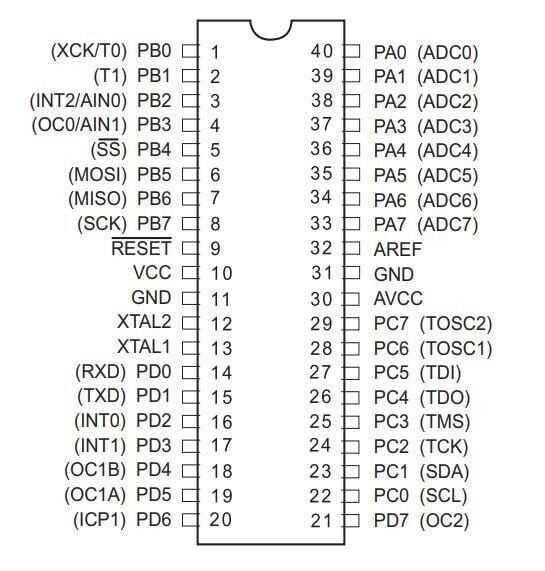
\includegraphics[width=0.75\textwidth]{atmega_sodo.png}
    \caption{Sơ đồ phân bố chân của vi điều khiển ATmega16 dạng đóng vỏ DIP-40}
    \label{fig:atmega16-pinout}
\end{figure}

Các thông số kỹ thuật then chốt của vi điều khiển ATmega16 được tổng hợp trong Bảng \ref{tab:atmega16-specs}:

\begin{table}[H]
\centering
\caption{Thông số kỹ thuật chính của vi điều khiển ATmega16}
\label{tab:atmega16-specs}
\begin{tabularx}{\textwidth}{>{\bfseries}p{5.0cm}X}
\toprule
Thông số & Giá trị định mức / Đặc tính kỹ thuật \\
\midrule
Kiến trúc CPU & 8-bit AVR RISC với 32 thanh ghi làm việc đa năng 8-bit \\
Bộ nhớ Flash chương trình & 16 Kbytes (In-System Reprogrammable Flash, độ bền 10.000 lần ghi/xóa) \\
Bộ nhớ SRAM nội & 1 Kbyte (1024 Bytes) \\
Bộ nhớ EEPROM nội & 512 Bytes (Lưu trữ dữ liệu không mất khi mất điện, độ bền 100.000 lần) \\
Tần số xung nhịp tối đa & 0 -- 16 MHz (Điện áp 4.5V -- 5.5V) \\
Số chân I/O khả trình & 32 chân chia làm 4 cổng 8-bit (PORT A, PORT B, PORT C, PORT D) \\
Bộ định thời / Bộ đếm (Timer) & 2 bộ Timer/Counter 8-bit và 1 bộ Timer/Counter 16-bit đa chức năng \\
Các kênh PWM & 4 kênh điều chế độ rộng xung phần cứng \\
Bộ chuyển đổi ADC & 8 kênh ADC 10-bit tích hợp sẵn trên PORT A \\
Giao tiếp truyền thông & USART, SPI, I2C/TWI \\
Giao diện gỡ lỗi phần cứng & Chuẩn JTAG (IEEE std. 1149.1) hỗ trợ On-Chip Debug \\
Điện áp hoạt động & 4.5V -- 5.5V đối với ATmega16 chuẩn (2.7V -- 5.5V đối với ATmega16L) \\
\bottomrule
\end{tabularx}
\end{table}

\subsection{Cấu trúc các cổng vào/ra và chức năng trong đồ án}

Vi điều khiển ATmega16 trang bị 32 chân vào ra hai chiều, được phân bổ đều cho 4 cổng ngoại vi ký hiệu từ A đến D. Mỗi cổng được kiểm soát độc lập bởi 3 thanh ghi điều khiển địa chỉ bộ nhớ:
\begin{itemize}[leftmargin=1.2cm]
    \item Thanh ghi DDRx (hướng dữ liệu): Thiết lập cấu hình hướng cho từng chân (Bit = 0: Chân là đầu vào Input; Bit = 1: Chân là đầu ra Output).
    \item Thanh ghi PORTx (dữ liệu xuất): Khi chân được thiết lập là Output, việc ghi 0 hoặc 1 vào bit tương ứng sẽ xuất điện áp mức thấp (0V) hoặc mức cao (5V). Khi chân là Input, ghi bit 1 sẽ kích hoạt điện trở kéo lên nội, ghi bit 0 sẽ đưa chân về trạng thái trở kháng cao.
    \item Thanh ghi PINx (đọc dữ liệu vào): Đọc trạng thái logic điện áp thực tế tại các chân cổng.
\end{itemize}

Trong đề tài, PA1 nối với chân dữ liệu của DHT11, PC4 -- PC7 và PD5 -- PD7 dùng cho LCD 1602, PD0 -- PD4 điều khiển 5 LED cảnh báo; bảng kết nối đầy đủ ở Bảng \ref{tab:hardware-wiring}.

\subsection{Xung nhịp hệ thống và phân tích xung đột ngoại vi JTAG}

\subsubsection{Cấu hình nguồn xung nhịp 8.0 MHz bằng Fuse Bits}
ATmega16 tích hợp sẵn mạch dao động RC nội đã hiệu chuẩn, có khả năng tạo ra các tần số xung nhịp cố định gồm 1.0 MHz, 2.0 MHz, 4.0 MHz và 8.0 MHz mà không đòi hỏi phải gắn thêm thạch anh dao động ngoài hay tụ lọc phụ trợ.

Sơ đồ kit có bố trí thạch anh ngoài \texttt{XT1} và hai tụ tải. Cấu hình phần mềm của đồ án chọn dao động RC nội 8.0 MHz, do đó không sử dụng khối thạch anh ngoài. Giá trị \texttt{F\_CPU = 8000000UL} chỉ phục vụ tính toán trễ khi biên dịch; tần số phần cứng được chọn bằng Fuse Bits. Fuse được ghi ở bước nạp chương trình bằng ProgISP (mục \ref{sec:progisp}, Hình \ref{fig:progisp-setup}) với cấu hình:
\begin{itemize}[leftmargin=1.2cm]
    \item Low Fuse Byte = \texttt{0xE4}: Thiết lập các bit \texttt{CKSEL3..0 = 0100} chọn mạch dao động RC nội 8.0 MHz, thời gian khởi động là 6 chu kỳ clock cộng trễ bổ sung điển hình 65 ms ở 5V (\texttt{SUT1..0 = 10}, Bảng 10 của datasheet).
\end{itemize}

\subsubsection{Phân tích xung đột phần cứng JTAG trên PORT C}
Mặc định khi xuất xưởng từ nhà sản xuất, bit cầu chì \texttt{JTAGEN} trên High Fuse Byte luôn được kích hoạt sẵn (\texttt{JTAGEN = 0}). Khi giao tiếp JTAG hoạt động, phần cứng vi điều khiển sẽ chiếm dụng cố định 4 chân trên cổng C:
\begin{itemize}[leftmargin=1.2cm]
    \item Chân PC2 = TCK (Test Clock)
    \item Chân PC3 = TMS (Test Mode Select)
    \item Chân PC4 = TDO (Test Data Output)
    \item Chân PC5 = TDI (Test Data Input)
\end{itemize}

Bus dữ liệu 4 bit của LCD 1602 nối vào PC4 -- PC7. Khi JTAG còn bật, hai chân PC4 và PC5 do khối gỡ lỗi điều khiển và không còn hoạt động như GPIO, nên LCD không nhận được chuỗi lệnh khởi tạo. Triệu chứng thường gặp là dòng 1 hiện toàn ô đen, dòng 2 để trống.

Để dùng PC4, PC5 cho LCD, đề tài tắt JTAG theo hai cách:
\begin{enumerate}[leftmargin=1.2cm]
    \item Tắt JTAG ở mức phần cứng: Cấu hình High Fuse Byte = \texttt{0xD9}. Tại giá trị này, bit 6 (\texttt{JTAGEN}) mang giá trị 1 (vô hiệu hóa JTAG), bit 5 (\texttt{SPIEN}) mang giá trị 0 (duy trì cổng nạp SPI để nạp code qua USBasp).
    \item Tắt JTAG ở mức phần mềm: Ghi bit \texttt{JTD} trên thanh ghi \texttt{MCUCSR} hai lần liên tiếp trong vòng 4 chu kỳ máy ngay ở đầu hàm \texttt{main()}:
    \begin{verbatim}
    MCUCSR = (1 << JTD);
    MCUCSR = (1 << JTD);
    \end{verbatim}
\end{enumerate}

\section{Mạch Kit thực hành vi điều khiển họ AVR}

Kit AVR sử dụng trong đồ án được triển khai từ sơ đồ nguyên lý do giảng viên cung cấp \cite{hust-kit-manual}. Nhóm vẽ lại sơ đồ và thiết kế PCB trên Altium Designer; bố trí linh kiện được thể hiện ở Hình \ref{fig:atmega-kit}.

\begin{figure}[H]
    \centering
    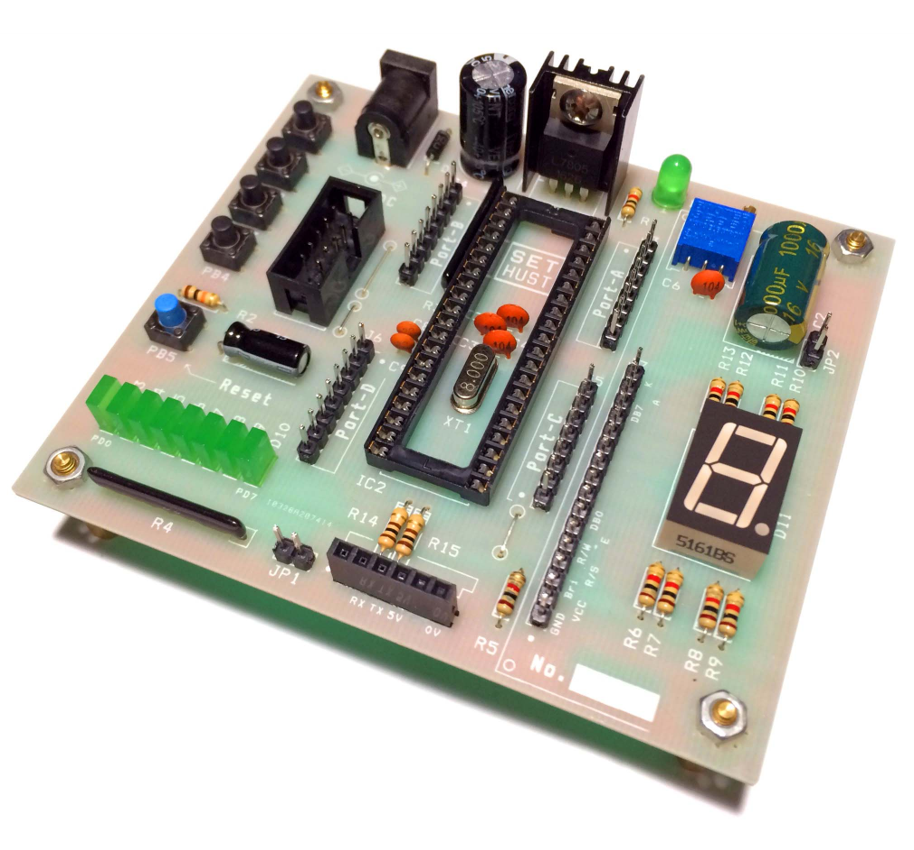
\includegraphics[width=0.78\textwidth]{atmega_kit_2d.png}
    \caption{Mô hình 3D bố trí linh kiện trên Kit phát triển vi điều khiển AVR}
    \label{fig:atmega-kit}
\end{figure}

Kit phát triển tích hợp đầy đủ các khối chức năng ngoại vi cơ bản:
\begin{enumerate}[leftmargin=1.2cm]
    \item Đế cắm vi điều khiển DIP-40: Cho phép lắp và thay thế vi điều khiển trong quá trình thực hành.
    \item Khối nguồn nuôi và ổn áp 5V: Tích hợp IC ổn áp tuyến tính LM7805 hạ áp từ nguồn Adapter ngoài DC 9V--12V, đồng thời hỗ trợ nhận nguồn 5V trực tiếp từ cổng USB qua mạch nạp USBasp, kết hợp hệ thống tụ lọc nguồn và đèn LED chỉ thị nguồn VCC.
    \item Giao diện nạp chương trình chuẩn ISP 10 chân (IDC-10): Kết nối trực tiếp với mạch nạp USBasp qua các đường tín hiệu MOSI (PB5), MISO (PB6), SCK (PB7), RESET và GND.
    \item Hàng rào cắm mở rộng J7 cho LCD 1602: Chuẩn cắm hàng đơn 16 chân tương thích với các màn hình chuẩn HD44780, tích hợp sẵn biến trở vi chỉnh VR1 dùng để điều chỉnh độ tương phản.
    \item Dàn LED đơn và phím bấm chức năng: Hệ thống 8 LED đơn nối về PORT D và ma trận nút bấm điều khiển nối về PORT B phục vụ các bài toán thực hành giao tiếp vào ra cơ bản. Đồ án dùng 5 LED trên PD0--PD4 để cảnh báo; 3 LED còn lại trên PD5--PD7 nằm chung đường với tín hiệu điều khiển LCD nên sẽ sáng theo mức logic của RW, RS, EN.
\end{enumerate}

\section{Cảm biến số nhiệt độ và độ ẩm DHT11}

\subsection{Cấu tạo và nguyên lý hoạt động}

DHT11 là cảm biến số đo nhiệt độ và độ ẩm môi trường tích hợp vi xử lý 8-bit hiệu năng cao bên trong để số hóa và hiệu chuẩn dữ liệu trước khi truyền ra ngoài \cite{dht11-datasheet}. Cấu tạo cảm biến bao gồm hai thành phần cảm nhận vật lý:
\begin{itemize}[leftmargin=1.2cm]
    \item Cảm biến độ ẩm kiểu điện trở: Sử dụng một phần tử màng polymer nhạy ẩm có các điện cực xen kẽ. Khi độ ẩm môi trường biến thiên, các phân tử hơi nước được hấp thụ vào bề mặt làm phân ly các ion dẫn, dẫn đến biến đổi điện trở của màng. Vi điều khiển 8-bit tích hợp bên trong DHT11 sẽ đo đạc sự thay đổi điện trở này và tính toán quy đổi thành giá trị độ ẩm tương đối (\%RH).
    \item Cảm biến nhiệt độ NTC: Là một điện trở nhiệt bán dẫn có hệ số nhiệt điện trở âm. Khi nhiệt độ môi trường tăng lên, điện trở của linh kiện giảm xuống theo một hàm phi tuyến được định trước. Vi điều khiển chuyển đổi giá trị điện trở này thành nhiệt độ thực tế theo thang đo độ Celsius ($^\circ\text{C}$).
\end{itemize}

\begin{table}[H]
\centering
\small
\caption{Đặc tính kỹ thuật của cảm biến số DHT11}
\label{tab:dht11-specs}
\begin{tabularx}{\textwidth}{>{\bfseries}p{5.0cm}X}
\toprule
Thông số kỹ thuật & Giá trị danh định \\
\midrule
Điện áp hoạt động & 3.0V -- 5.5V DC (theo bản tài liệu tham chiếu) \\
Dải đo nhiệt độ & $0^\circ\text{C}$ -- $50^\circ\text{C}$ \\
Độ chính xác đo nhiệt độ & $\pm 2.0^\circ\text{C}$ \\
Độ phân giải nhiệt độ & $1.0^\circ\text{C}$ (bản DHT11 trong tài liệu tham chiếu) \\
Dải đo độ ẩm & 20\% -- 90\% RH \\
Độ chính xác đo độ ẩm & $\pm 5.0\%$ RH \\
Độ phân giải độ ẩm & 1\% RH \\
Khoảng cách giữa các lần đọc & Tối thiểu 1 giây theo bản tài liệu tham chiếu; chương trình chọn trễ 2 giây mỗi vòng lặp \\
Dòng điện tiêu thụ & $0.5\text{ mA} - 2.5\text{ mA}$ khi đo; $100\text{ }\mu\text{A} - 150\text{ }\mu\text{A}$ khi chờ \\
Chuẩn giao tiếp & Aosong 1-Wire Single-Bus (Đường truyền đơn tuyến chuyên biệt) \\
\bottomrule
\end{tabularx}
\end{table}

Module sử dụng trong mô hình là loại DHT11 gắn trên PCB, đầu nối 3 chân, mã bán hàng \texttt{LK\_02463}. Mã này không xác định phiên bản chip hoặc bản datasheet. Khi đấu nối cần dựa trên nhãn VCC, DATA (hoặc S) và GND trên module, không áp dụng trực tiếp số chân của cảm biến rời 4 chân. Bảng \ref{tab:dht11-specs} dùng làm cơ sở tham chiếu cho DHT11. Chương trình hiển thị trực tiếp Byte 2 ($T_{int}$) và Byte 3 ($T_{dec}$) lên LCD, nên các giá trị $26.5^\circ\text{C}$ và $31.5^\circ\text{C}$ ghi nhận ở Chương 3 cho thấy module thực tế trả về byte thập phân khác 0, khác với mức phân giải $1^\circ\text{C}$ của bản tài liệu tham chiếu.

\subsection{Giao thức truyền thông đơn tuyến Aosong 1-Wire}
\label{sec:dht11-protocol}

\textbf{Phân định chuẩn giao thức}: Giao thức truyền thông một dây (Single-Bus) của DHT11 do nhà sản xuất Aosong thiết kế là giao thức điểm--điểm chuyên biệt, \textbf{không tương thích} với chuẩn công nghiệp Dallas/Maxim 1-Wire (vốn sử dụng mã định danh ROM 64-bit, khe thời gian do Master chủ động điều khiển và hỗ trợ kết nối đa điểm trên cùng một bus). Giao thức của DHT11 hoạt động theo nguyên tắc Master phát xung khởi động kích hoạt một lần, sau đó Slave (cảm biến) tự động phát liên tục chuỗi 40 bit dữ liệu theo các mốc thời gian quy ước.

Cảm biến DHT11 giao tiếp với vi điều khiển chỉ thông qua một chân dữ liệu DATA duy nhất. Đường tín hiệu này đòi hỏi phải có một điện trở kéo lên nguồn 5V (giá trị từ 4.7 k$\Omega$ đến 10 k$\Omega$) để duy trì mức cao khi đường truyền ở trạng thái rảnh rỗi.

Toàn bộ quy trình trao đổi dữ liệu một lần đọc (gồm 40 bit) tuân theo trình tự định thì thời gian nghiêm ngặt được mô tả dưới đây:

\subsubsection{1. Tín hiệu khởi động}
Vi điều khiển phát tín hiệu khởi động:
\begin{itemize}[leftmargin=1.2cm]
    \item MCU cấu hình chân PA1 thành Output và kéo đường bus xuống mức LOW trong thời gian tối thiểu 18 ms (trong chương trình chọn trễ an toàn là \texttt{\_delay\_ms(20)}).
    \item MCU sau đó giải phóng quyền điều khiển bus bằng cách chuyển chân PA1 sang chế độ Input và kích hoạt điện trở kéo lên nội, tạo khoảng trễ 30 $\mu$s để đường tín hiệu được kéo lên mức HIGH an toàn trước khi cảm biến bắt đầu phản hồi. Việc chuyển sang đầu vào cho phép cảm biến điều khiển đường DATA mà không bị MCU chủ động giữ mức cao.
\end{itemize}

\subsubsection{2. Tín hiệu phản hồi từ cảm biến}
Khi nhận diện được xung khởi động hợp lệ, DHT11 sẽ kéo đường bus xuống mức LOW trong khoảng 80 $\mu$s, tiếp theo kéo lên mức HIGH trong 80 $\mu$s để thông báo đã sẵn sàng truyền gói dữ liệu.

\subsubsection{3. Thu nhận và giải mã 40 bit dữ liệu}
Sau khi gửi tín hiệu phản hồi, DHT11 bắt đầu tuần tự phát ra 40 bit nhị phân (chia đều thành 5 byte). Mỗi bit dữ liệu luôn được bắt đầu bằng một xung mức LOW kéo dài cố định khoảng 50 $\mu$s. Giá trị của bit nhị phân được mã hóa dựa trên độ rộng thời gian tồn tại của xung mức HIGH tiếp theo đó:
\begin{itemize}[leftmargin=1.2cm]
    \item Bit '0': Xung mức HIGH tồn tại trong khoảng từ 26 $\mu$s đến 28 $\mu$s.
    \item Bit '1': Xung mức HIGH tồn tại kéo dài trong khoảng 70 $\mu$s.
\end{itemize}

Cách vi điều khiển phân biệt hai độ rộng xung này được trình bày ở mục \ref{sec:dht11-read}.

\subsubsection{4. Cấu trúc gói tin và cơ chế kiểm tra lỗi}
Gói dữ liệu hoàn chỉnh gồm 5 byte (40 bit) truyền đi theo thứ tự:
\begin{equation}
\begin{aligned}
    \text{Gói dữ liệu} = \{ & \text{Byte 0: } RH_{int}, \quad \text{Byte 1: } RH_{dec}, \\
                            & \text{Byte 2: } T_{int}, \quad \text{Byte 3: } T_{dec}, \quad \text{Byte 4: } Checksum \}
\end{aligned}
\end{equation}

Byte cuối cùng là byte kiểm tra lỗi Checksum được tạo bởi tổng đại số của 4 byte dữ liệu trước đó (lấy 8 bit thấp):
\begin{equation}
    Checksum_{valid} = (RH_{int} + RH_{dec} + T_{int} + T_{dec}) \ \& \ \text{0xFF}
\end{equation}

Nếu giá trị tính toán trùng khớp với Byte 4 nhận được từ cảm biến, gói dữ liệu được xác nhận là hợp lệ. Thuật toán Checksum 8-bit giúp phát hiện hiệu quả các trường hợp méo dạng xung hoặc sai lệch bit đơn lẻ trên đường truyền; tuy nhiên, phương pháp tổng kiểm tra cộng 8-bit không có khả năng sửa lỗi và không thể loại trừ hoàn toàn các lỗi đảo bit bù trừ đa điểm.

\section{Màn hình hiển thị tinh thể lỏng LCD 1602}

Màn hình LCD 1602 là mô-đun hiển thị ký tự gồm 2 hàng, mỗi hàng có khả năng hiển thị tối đa 16 ký tự ma trận điểm $5 \times 8$ pixels, sử dụng vi mạch điều khiển tiêu chuẩn công nghiệp Hitachi HD44780 \cite{hd44780-datasheet}.

\begin{table}[H]
\centering
\caption{Bảng ánh xạ kết nối chân giữa giắc J7 trên Kit, màn hình LCD 1602 và ATmega16}
\label{tab:lcd-pinout}
\begin{tabularx}{\textwidth}{c c c >{\bfseries}c X}
\toprule
Chân J7 & Chân LCD & Tên chân & Chân MCU & Chức năng kỹ thuật \\
\midrule
1 & 1 & $V_{SS}$ & GND & Cực âm nguồn nuôi (0V) \\
2 & 2 & $V_{DD}$ & VCC & Cực dương nguồn nuôi (+5V) \\
3 & 3 & $V_0$ & VR1 & Điện áp điều chỉnh độ tương phản hiển thị màn hình \\
4 & 4 & RS & PD6 & Chọn thanh ghi (0: Thanh ghi Lệnh; 1: Thanh ghi Dữ liệu) \\
5 & 5 & RW & PD5 & Chọn chiều Đọc/Ghi (0: Ghi dữ liệu vào LCD; 1: Đọc từ LCD) \\
6 & 6 & E & PD7 & Chốt xung kích hoạt (Enable Strobe, tích cực sườn âm) \\
7 -- 10 & 7 -- 10 & D0 -- D3 & PC0 -- PC3 & 4 bit dữ liệu thấp (Không dùng ở chế độ 4-bit bus) \\
11 & 11 & D4 & PC4 & Bit dữ liệu D4 \\
12 & 12 & D5 & PC5 & Bit dữ liệu D5 \\
13 & 13 & D6 & PC6 & Bit dữ liệu D6 \\
14 & 14 & D7 & PC7 & Bit dữ liệu D7 \\
15 & 15 & A (LED+) & VCC & Cực anot đèn nền \\
16 & 16 & K (LED-) & GND & Cực katot đèn nền \\
\bottomrule
\end{tabularx}
\end{table}

Để tối ưu hóa số lượng chân vi điều khiển, đồ án áp dụng chế độ truyền thông 4-bit bus:
\begin{itemize}[leftmargin=1.2cm]
    \item Vi điều khiển chỉ cần dùng 4 chân GPIO (PC4 -- PC7) nối tới các chân dữ liệu D4 -- D7 của LCD, tiết kiệm được 4 chân so với chế độ 8-bit truyền thống.
    \item Mỗi byte dữ liệu hoặc mã lệnh 8-bit sẽ được tách làm hai nửa byte: 4 bit cao được truyền trước kèm theo một xung chốt Enable trên chân PD7, tiếp theo 4 bit thấp được dịch sang và truyền kèm theo một xung chốt Enable thứ hai.
\end{itemize}

\section{Khối cảnh báo và chỉ thị LED}

Dàn 5 đèn LED cảnh báo trên Kit thí nghiệm được nối trực tiếp vào các chân từ PD0 đến PD4 của cổng D. Mạch được thiết kế theo cấu hình tích cực mức thấp (Active Low):
\begin{itemize}[leftmargin=1.2cm]
    \item Cực Anot của các đèn LED được cấp nguồn dương VCC qua mạng điện trở hạn dòng R4 và jumper JP1. Trên sơ đồ kit, R4 được ghi giá trị 10 k$\Omega$.
    \item Cực Katot của các đèn LED nối về các chân vi điều khiển PD0 -- PD4.
    \item Khi vi điều khiển xuất mức 0 (mức thấp): Dòng điện chạy từ VCC qua LED xuống chân vi điều khiển khép mạch, LED bật sáng (báo động vượt ngưỡng).
    \item Khi vi điều khiển xuất mức 1 (mức cao): Không có chênh lệch điện áp qua diode, LED tắt (trạng thái không cảnh báo quá nhiệt).
\end{itemize}

\chapter{THIẾT KẾ VÀ TRIỂN KHAI HỆ THỐNG}
\begingroup
\clubpenalty=10000
\widowpenalty=10000
\setlength{\parskip}{4pt}
\setlist{itemsep=2pt,parsep=0pt,topsep=3pt}

\section{Yêu cầu thiết kế và lựa chọn linh kiện}
\label{sec:requirements}

\subsection{Yêu cầu của hệ thống}

Từ tên đề tài và điều kiện thực hiện trên kit AVR của học phần, nhóm đặt ra các yêu cầu thiết kế trong Bảng \ref{tab:requirements}. Vi điều khiển ATmega16 có sẵn trên kit nên không thuộc phạm vi lựa chọn; các mục tiếp theo trình bày việc chọn cảm biến và thiết bị hiển thị, cảnh báo.

\begin{table}[H]
\centering
\small
\caption{Yêu cầu thiết kế của hệ thống}
\label{tab:requirements}
\renewcommand{\arraystretch}{1.15}
\begin{tabularx}{\textwidth}{>{\bfseries\raggedright\arraybackslash}p{2.3cm} >{\raggedright\arraybackslash}X >{\raggedright\arraybackslash}p{4.2cm}}
\toprule
Nhóm yêu cầu & Chỉ tiêu & Cách đáp ứng \\
\midrule
Đo nhiệt độ & Nhiệt độ môi trường trong phòng, dải tối thiểu 0--50\,$^\circ$C; cập nhật khoảng 2 giây một lần & DHT11 (mục \ref{sec:sensor-choice}); chu kỳ đọc (mục \ref{sec:threshold}) \\
Hiển thị & Hiện giá trị đo, ngưỡng và thông báo lỗi bằng chữ ngay trên mô hình & LCD 1602 (mục \ref{sec:display-choice}) \\
Cảnh báo & Báo khi nhiệt độ đạt hoặc vượt 30\,$^\circ$C bằng tín hiệu nhìn thấy được; tự trở về khi nhiệt độ giảm & 5 LED trên PD0--PD4 (mục \ref{sec:threshold}) \\
Độ tin cậy & Phát hiện mất tín hiệu và gói tin sai; vi điều khiển không bị treo khi cảm biến hỏng & Timeout và checksum (mục \ref{sec:dht11-read}) \\
Phần cứng & Dùng kit ATmega16 có sẵn, nguồn 5\,V, nạp qua USBasp; hạn chế linh kiện ngoài kit & Kết nối ở Bảng \ref{tab:hardware-wiring} \\
\bottomrule
\end{tabularx}
\end{table}

\subsection{Lựa chọn cảm biến nhiệt độ}
\label{sec:sensor-choice}

Bảng \ref{tab:sensor-compare} so sánh ba cảm biến nhiệt độ phổ biến khi làm việc với vi điều khiển AVR \cite{dht11-datasheet,lm35-datasheet,ds18b20-datasheet}.

\begin{table}[H]
\centering
\small
\caption{So sánh các phương án cảm biến nhiệt độ}
\label{tab:sensor-compare}
\renewcommand{\arraystretch}{1.15}
\setlength{\tabcolsep}{4pt}
\begin{tabularx}{\textwidth}{>{\bfseries\raggedright\arraybackslash}p{2.6cm} >{\raggedright\arraybackslash}X >{\raggedright\arraybackslash}X >{\raggedright\arraybackslash}X}
\toprule
Tiêu chí & LM35 & DS18B20 & DHT11 \\
\midrule
Tín hiệu ra & Điện áp tương tự, 10\,mV/$^\circ$C & Số, bus 1-Wire (Dallas) & Số, Single-Bus (Aosong) \\
Dải đo nhiệt độ & $-55$ đến 150\,$^\circ$C & $-55$ đến 125\,$^\circ$C & 0 đến 50\,$^\circ$C \\
Độ chính xác & 0,5\,$^\circ$C tại 25\,$^\circ$C & $\pm$0,5\,$^\circ$C trong khoảng $-10$ đến 85\,$^\circ$C & $\pm$2\,$^\circ$C \\
Độ phân giải & Phụ thuộc ADC: khoảng 0,49\,$^\circ$C với ADC 10 bit, tham chiếu 5\,V & 0,5 đến 0,0625\,$^\circ$C (9--12 bit) & 1\,$^\circ$C theo tài liệu tham chiếu \\
Nguồn cấp & 4--30\,V & 3,0--5,5\,V & 3,0--5,5\,V \\
Thời gian đọc & Một lần chuyển đổi ADC & Tối đa 750\,ms ở 12 bit & Khoảng 25\,ms; hai lần đọc cách nhau tối thiểu 1\,s \\
Đo độ ẩm & Không & Không & Có (20--90\,\% RH) \\
Kết nối với MCU & Một kênh ADC; dây tín hiệu tương tự dễ nhiễm nhiễu & Một chân GPIO, điện trở kéo lên & Một chân GPIO, điện trở kéo lên \\
\bottomrule
\end{tabularx}
\end{table}

LM35 và DS18B20 chính xác hơn DHT11. Nhóm vẫn chọn DHT11 vì các lý do sau:
\begin{itemize}[leftmargin=1.2cm]
    \item Dải 0--50\,$^\circ$C và sai số $\pm$2\,$^\circ$C đáp ứng yêu cầu cảnh báo ngưỡng 30\,$^\circ$C trong phòng ở Bảng \ref{tab:requirements}.
    \item Tín hiệu số chỉ cần một chân GPIO (PA1); không chiếm kênh ADC và không phụ thuộc điện áp tham chiếu hay nhiễu trên dây như LM35.
    \item Module 3 chân dễ đấu nối ngoài kit; cảm biến đo thêm độ ẩm, cho phép mở rộng chức năng mà không đổi phần cứng.
    \item Giao thức buộc chương trình tự tạo và lấy mẫu xung theo thời gian, phù hợp với nội dung lập trình thanh ghi của học phần.
\end{itemize}
Đổi lại, sai số của DHT11 lớn hơn hai phương án còn lại. Nếu ứng dụng cần độ chính xác cao hơn, DS18B20 có thể thay trên cùng chân PA1, với thay đổi chủ yếu ở phần mềm giao tiếp.

\subsection{Lựa chọn thiết bị hiển thị và cảnh báo}
\label{sec:display-choice}

Kit có sẵn ba thiết bị đầu ra dùng được: LED 7 thanh một chữ số D11, dãy 8 LED đơn trên PORT D và giắc J7 dành cho LCD 1602 (Hình \ref{fig:schematic}). LED 7 thanh một chữ số không đủ để hiện giá trị như \texttt{26.5} hay các thông báo lỗi, đồng thời dùng chung PC0--PC7 với giắc LCD. Nhóm chọn LCD 1602 (2 dòng $\times$ 16 ký tự, bộ điều khiển HD44780) vì đủ chỗ cho giá trị đo, ngưỡng và thông báo chẩn đoán bằng chữ; LCD chạy ở chế độ 4 bit để chỉ chiếm PC4--PC7 và PD5--PD7.

Khối cảnh báo dùng 5 LED đơn trên PD0--PD4: các LED có sẵn trên kit, không cần mạch ngoài và dễ quan sát. Còi báo không có trên kit nên được đưa vào hướng phát triển (mục \ref{sec:future}).

\section{Thiết kế kiến trúc phần cứng và sơ đồ nguyên lý}

\subsection{Sơ đồ khối chức năng và kết nối liên khối hệ thống}

Nhóm vẽ lại sơ đồ giảng viên cung cấp (Hình \ref{fig:schematic}) \cite{hust-kit-manual} và thiết kế PCB trên Altium Designer (Hình \ref{fig:altium-3d}). DHT11 nối ngoài kit theo Hình \ref{fig:system-wiring}. Hệ thống gồm 5 khối chức năng:
\begin{enumerate}[leftmargin=1.2cm, topsep=0pt, itemsep=0.5pt, parsep=0pt]
    \item \textbf{Khối nguồn nuôi 5V}: Cung cấp điện áp +5V ổn định cho toàn mạch qua IC LM7805 hoặc qua cổng USB máy tính.
    \item \textbf{Khối MCU trung tâm}: ATmega16 (DIP-40, dao động nội 8.0 MHz) đảm nhiệm điều phối toàn bộ chu trình hoạt động.
    \item \textbf{Khối cảm biến}: Cảm biến DHT11 thu thập giá trị nhiệt độ và độ ẩm, giao tiếp đơn tuyến với MCU qua chân PA1.
    \item \textbf{Khối hiển thị}: Màn hình LCD 1602 giao tiếp 4-bit qua các chân dữ liệu PC4--PC7 và chân điều khiển PD5--PD7.
    \item \textbf{Khối cảnh báo}: Dàn 5 LED đơn nối với chân PD0--PD4, tích cực mức thấp qua mạng điện trở R4 trên kit.
\end{enumerate}

\begin{figure}[H]\vspace{-0.25cm}
    \centering
    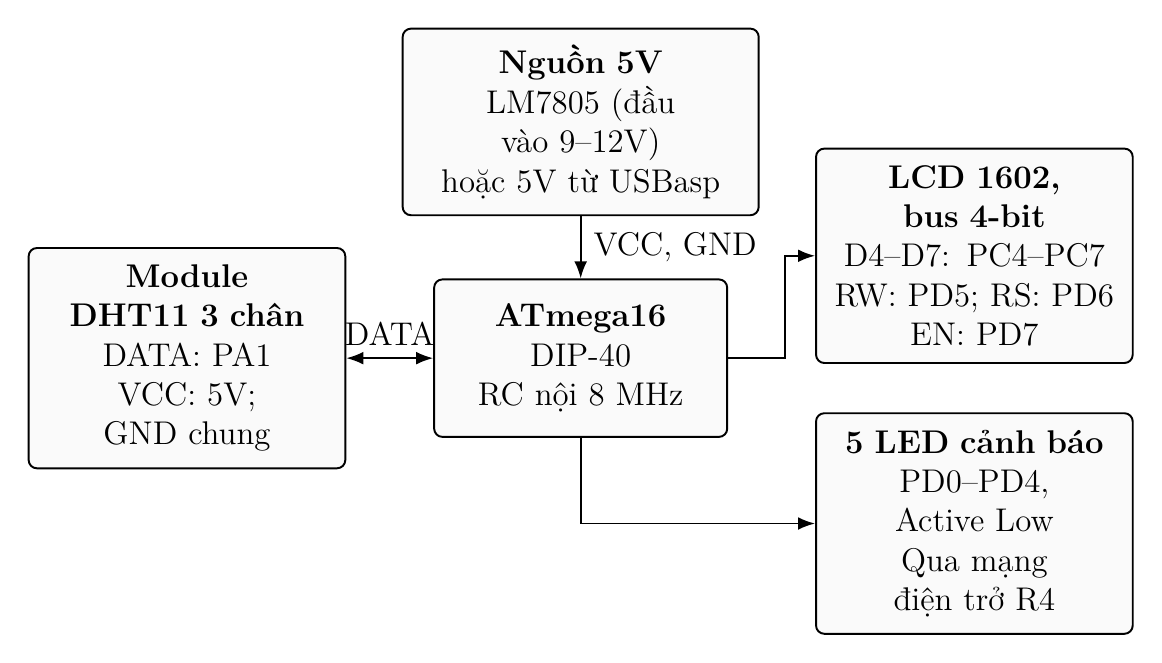
\begin{tikzpicture}[
    font=\small, >=Latex, line width=0.7pt,
    block/.style={draw, rounded corners=3pt, align=center, minimum height=1.5cm, text width=3.6cm, inner sep=6pt, fill=gray!4}
]
\node[block,text width=4.1cm] (power) at (0,0) {\textbf{Nguồn 5V}\\LM7805 (đầu vào 9--12V)\\hoặc 5V từ USBasp};
\node[block,text width=3.3cm,minimum height=2cm] (mcu) at (0,-3.0) {\textbf{ATmega16}\\DIP-40\\RC nội 8 MHz};
\node[block] (dht) at (-5.0,-3.0) {\textbf{Module DHT11 3 chân}\\DATA: PA1\\VCC: 5V; GND chung};
\node[block] (lcd) at (5.0,-1.7) {\textbf{LCD 1602, bus 4-bit}\\D4--D7: PC4--PC7\\RW: PD5; RS: PD6\\EN: PD7};
\node[block] (led) at (5.0,-5.1) {\textbf{5 LED cảnh báo}\\PD0--PD4, Active Low\\Qua mạng điện trở R4};
\draw[->] (power.south) -- node[right]{VCC, GND} (mcu.north);
\draw[<->] (dht.east) -- node[above]{DATA} (mcu.west);
\draw[->] (mcu.east) -- (2.6,-3.0) |- (lcd.west);
\draw[->] (mcu.south) -- (0,-5.1) -- (led.west);
\end{tikzpicture}
\vspace{-0.2cm}
    \caption{Sơ đồ kết nối liên khối chi tiết của hệ thống đo nhiệt độ và cảnh báo}
    \label{fig:system-wiring}
\end{figure}

% Sơ đồ gốc (img/schematic.png) được tách tại khoảng trống dọc giữa khối MCU và
% ba khối bên phải; các khối nối với nhau qua nhãn mạng nên không cắt qua dây nối.
\begin{figure}[p]
    \centering
    \begin{subfigure}{\textwidth}
        \centering
        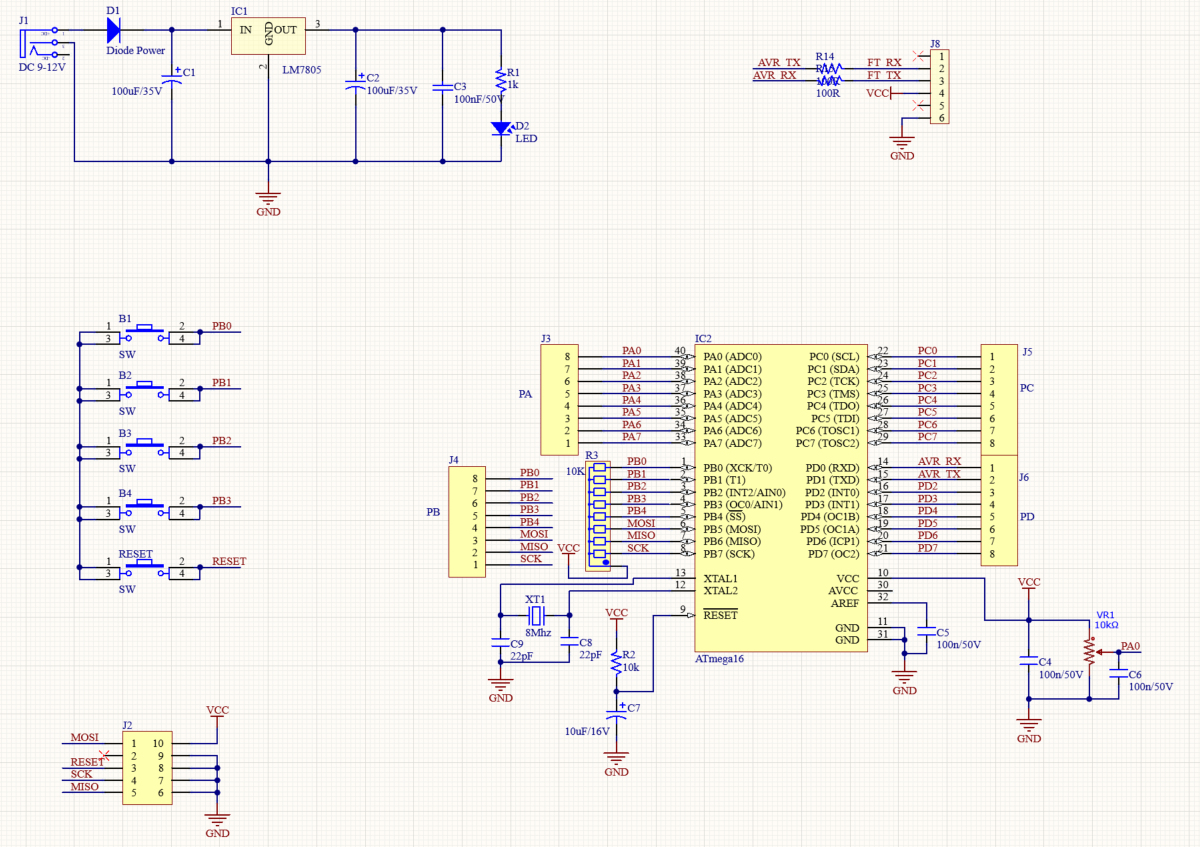
\includegraphics[width=\textwidth]{schematic_main.png}
        \caption{Khối nguồn, vi điều khiển ATmega16, nút bấm, cổng nạp ISP (J2) và các giắc mở rộng cổng}
        \label{fig:schematic-main}
    \end{subfigure}

    \vspace{0.5cm}
    \begin{subfigure}[b]{5.36cm}
        \centering
        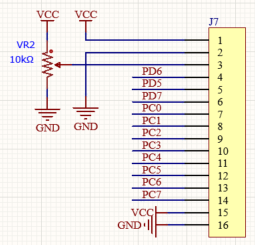
\includegraphics[width=\linewidth]{schematic_lcd.png}
        \caption{Giắc J7 nối LCD 1602}
        \label{fig:schematic-lcd}
    \end{subfigure}\hfill
    \begin{subfigure}[b]{4.31cm}
        \centering
        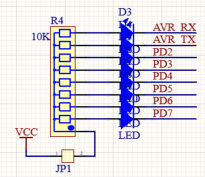
\includegraphics[width=\linewidth]{schematic_led.png}
        \caption{Dãy LED đơn}
        \label{fig:schematic-led}
    \end{subfigure}\hfill
    \begin{subfigure}[b]{5.71cm}
        \centering
        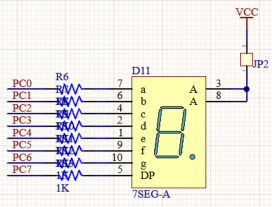
\includegraphics[width=\linewidth]{schematic_7seg.png}
        \caption{LED 7 thanh}
        \label{fig:schematic-7seg}
    \end{subfigure}

    \vspace{0.3cm}
    \caption{Sơ đồ nguyên lý kit AVR được nhóm vẽ lại từ tài liệu giảng viên cung cấp}
    \label{fig:schematic}
    \vspace{0.1cm}
    {\small\textit{Ghi chú:} Các khối (a)--(d) nối với nhau qua nhãn mạng (PA0--PD7, VCC, GND). Trong đồ án, LCD dùng PC4--PC7 và PD5--PD7; 5 LED cảnh báo dùng PD0--PD4. Khối thạch anh XT1 có trên sơ đồ nhưng chương trình chọn dao động RC nội 8 MHz. Cảm biến DHT11 là module nối ngoài, không nằm trong sơ đồ kit này.\par}
\end{figure}

\subsection{Bảng kết nối dây chi tiết giữa các linh kiện}

Bảng \ref{tab:hardware-wiring} liệt kê kết nối giữa từng khối chức năng và chân của ATmega16; số chân tính theo vỏ DIP-40 (Hình \ref{fig:atmega16-pinout}). Tên tín hiệu sau dấu ``/'' là chức năng thay thế của chân, không được dùng trong đồ án.

\begin{table}[tb]
\centering
\small
\caption{Bảng tổng hợp kết nối tín hiệu phần cứng của hệ thống}
\label{tab:hardware-wiring}
\renewcommand{\arraystretch}{1.08}
\setlength{\tabcolsep}{3pt}
\begin{tabularx}{\textwidth}{>{\bfseries\raggedright\arraybackslash}p{2.1cm} >{\raggedright\arraybackslash}p{2.5cm} >{\centering\arraybackslash}p{1.7cm} >{\bfseries\raggedright\arraybackslash}p{2.6cm} >{\raggedright\arraybackslash}X}
\toprule
Khối chức năng & Chân linh kiện & Chân MCU & Tên tín hiệu MCU & Chức năng kỹ thuật \\
\midrule
Cảm biến DHT11 & DATA / S & Chân 39 & PA1 / ADC1 & Giao tiếp Single-Bus hai chiều \\
               & VCC & -- & +5V của kit & Nguồn nuôi +5V DC \\
               & GND & -- & GND của kit & Nối đất chung \\
\midrule
Màn hình LCD   & RS (Chân 4)  & Chân 20 & PD6 / ICP1 & Chọn thanh ghi (0: lệnh, 1: dữ liệu) \\
               & RW (Chân 5)  & Chân 19 & PD5 / OC1A & Chọn đọc/ghi (0: ghi) \\
               & EN (Chân 6)  & Chân 21 & PD7 / OC2 & Xung kích hoạt chốt dữ liệu \\
               & D4 (Chân 11) & Chân 26 & PC4 / TDO & Đường truyền dữ liệu bit 4 \\
               & D5 (Chân 12) & Chân 27 & PC5 / TDI & Đường truyền dữ liệu bit 5 \\
               & D6 (Chân 13) & Chân 28 & PC6 / TOSC1 & Đường truyền dữ liệu bit 6 \\
               & D7 (Chân 14) & Chân 29 & PC7 / TOSC2 & Đường truyền dữ liệu bit 7 \\
\midrule
Dàn LED cảnh báo & Katot LED 1 & Chân 14 & PD0 / RXD & Cảnh báo, sáng khi mức 0 \\
               & Katot LED 2 & Chân 15 & PD1 / TXD & Cảnh báo, sáng khi mức 0 \\
               & Katot LED 3 & Chân 16 & PD2 / INT0 & Cảnh báo, sáng khi mức 0 \\
               & Katot LED 4 & Chân 17 & PD3 / INT1 & Cảnh báo, sáng khi mức 0 \\
               & Katot LED 5 & Chân 18 & PD4 / OC1B & Cảnh báo, sáng khi mức 0 \\
\bottomrule
\end{tabularx}
\end{table}

\begin{figure}[tb]
    \centering
    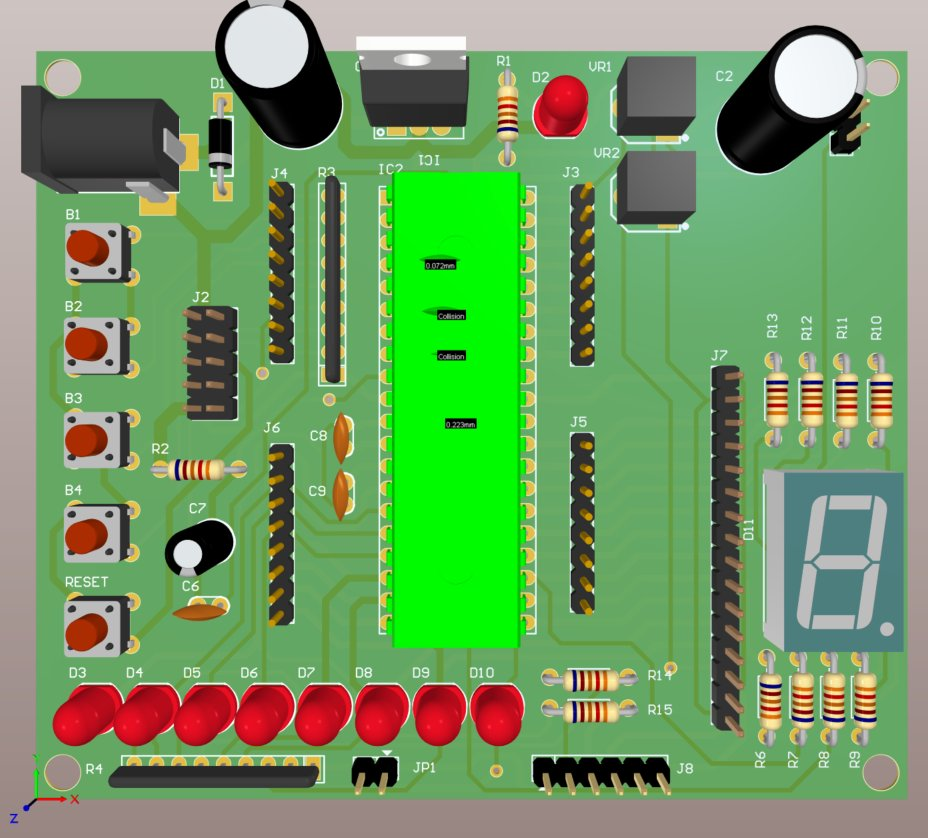
\includegraphics[width=0.48\textwidth]{atmega_kit_3d.png}
    \caption{Mô hình 3D PCB của nhóm trên Altium Designer}
    \label{fig:altium-3d}
\end{figure}

\section{Xây dựng thuật toán và phần mềm điều khiển}

\subsection{Thuật toán điều khiển tổng quát chương trình}
\label{sec:main-algo}

Chương trình vận hành tuần tự theo các bước dưới đây. Lưu đồ ở Hình \ref{fig:main-flowchart} thể hiện cùng các nhánh xử lý; mã nguồn đầy đủ nằm ở Phụ lục A.

\begin{enumerate}[leftmargin=0.8cm,itemsep=6pt,parsep=0pt,topsep=4pt]
    \item \textbf{Khởi tạo hệ thống.} Ghi hai lần bit JTD trong \texttt{MCUCSR} để tắt JTAG và giải phóng PC4, PC5. Khởi tạo LCD bằng \texttt{LCD4\_INIT}; đặt PD0--PD4 làm đầu ra (\texttt{DDRD |= 0x1F}) và xuất mức cao để tắt LED (\texttt{PORTD |= 0x1F}). LCD hiện \texttt{DA2: DO NHIET DO} và \texttt{DHT11 SENSOR} khoảng 1,5 giây, sau đó được xóa.
    \item \textbf{Đọc cảm biến.} Gọi \texttt{DHT11\_Read} để nhận dữ liệu nhiệt độ cùng mã trả về \texttt{status}. Chương trình chỉ so sánh ngưỡng và hiển thị nhiệt độ khi \texttt{status == 0}.
    \item \textbf{Xử lý dữ liệu hợp lệ.} Dòng 1 LCD hiển thị nhiệt độ theo định dạng \texttt{Temp: XX.Y °C}. Dòng 2 hiển thị ngưỡng; các khoảng trắng cuối chuỗi được dùng để ghi đè nội dung cũ trong 16 vị trí:
    \begin{itemize}[leftmargin=0.6cm,itemsep=3pt,topsep=3pt]
        \item Nếu \texttt{temp\_int >= 30}: hiện \texttt{HIGH Th: 30°C *!}; dùng \texttt{PORTD \&= 0xE0} kéo PD0--PD4 xuống mức thấp, bật 5 LED.
        \item Nếu \texttt{temp\_int < 30}: hiện \texttt{HIGH Th: 30°C}, xóa dấu \texttt{*!}; dùng \texttt{PORTD |= 0x1F} tắt 5 LED.
    \end{itemize}
    \item \textbf{Xử lý lỗi.} Không dùng lại dữ liệu cũ để so sánh ngưỡng. Cả hai nhánh lỗi đều tắt 5 LED bằng \texttt{PORTD |= 0x1F}:
    \begin{itemize}[leftmargin=0.6cm,itemsep=3pt,topsep=3pt]
        \item \texttt{status == -6}: hiện \texttt{DHT11: Sum Error} và \texttt{Checksum Invalid} trên hai dòng LCD.
        \item \texttt{status} từ -1 đến -5: hiện \texttt{DHT11: No Signal} và \texttt{Check Pin PA1}, tương ứng với timeout khi chờ tín hiệu.
    \end{itemize}
    Việc tắt LED khi lỗi tránh cảnh báo dựa trên dữ liệu cũ, nhưng cũng làm hệ thống không cảnh báo được nếu môi trường đang quá nhiệt; hạn chế này được nêu ở mục \ref{sec:conclusion-limits}.
    \item \textbf{Lặp lại.} Thực hiện \texttt{\_delay\_ms(2000)}, rồi quay lại bước đọc cảm biến. Thời gian giữa hai lượt đọc còn bao gồm giao tiếp và cập nhật LCD, như phân tích ở mục \ref{sec:threshold}.
\end{enumerate}

\begin{figure}[p]
\centering
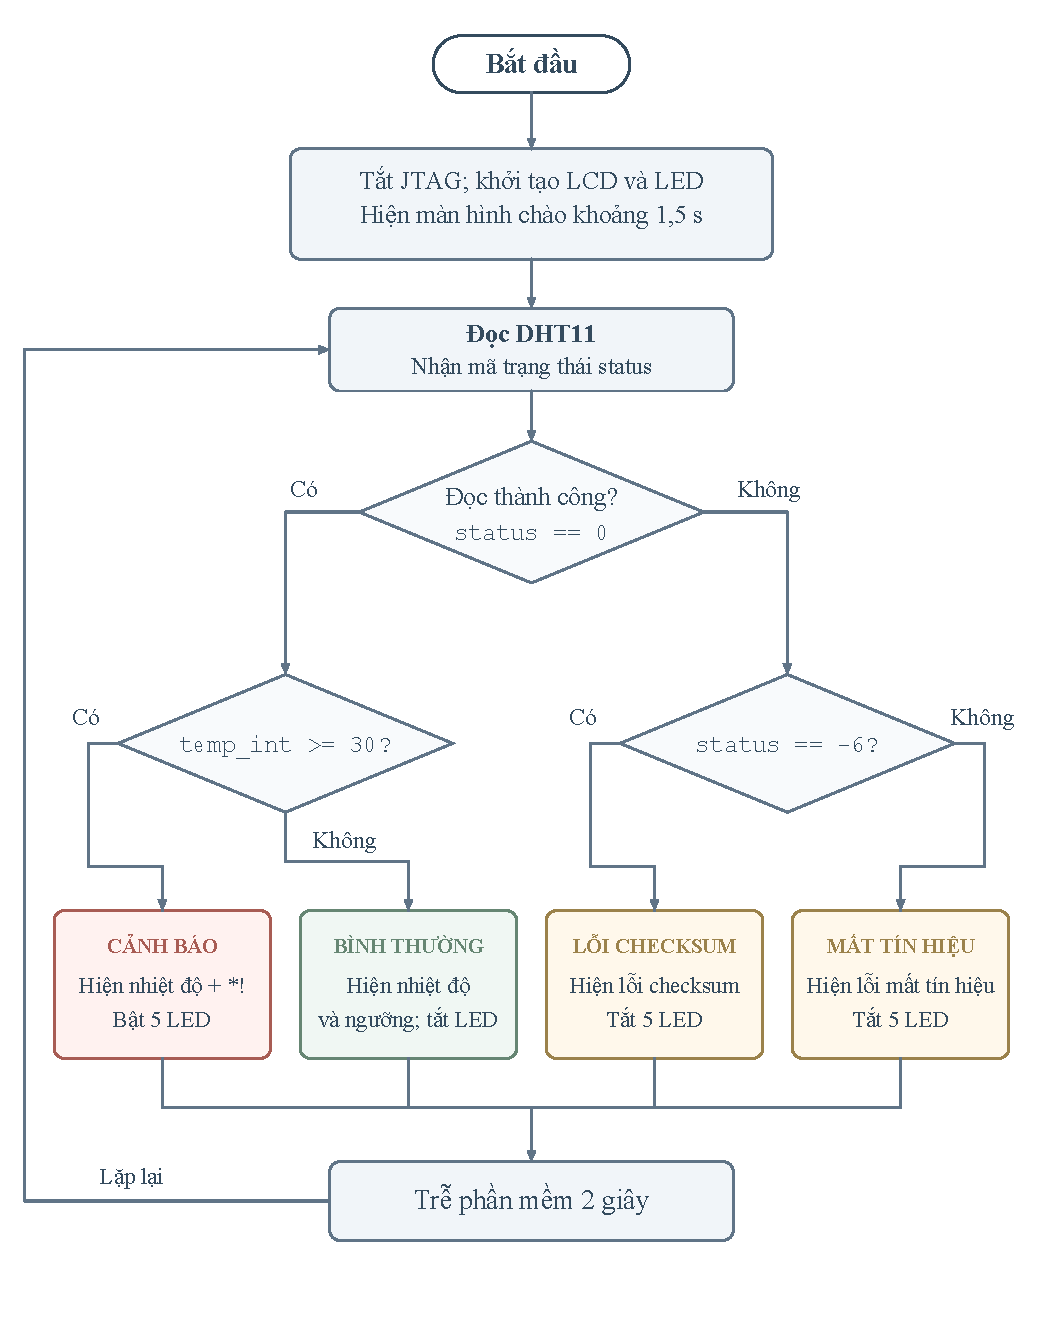
\includegraphics[width=\textwidth,height=0.88\textheight,keepaspectratio]{diagrams/main-flowchart.pdf}
\caption{Lưu đồ thuật toán đo nhiệt độ, cảnh báo và xử lý lỗi}
\label{fig:main-flowchart}
\end{figure}

\subsection{Thuật toán giao tiếp và giải mã cảm biến DHT11}
\label{sec:dht11-read}

Hàm \texttt{DHT11\_Read(uint8\_t *temp\_int, uint8\_t *temp\_dec, uint8\_t *humi\_int)} được viết trực tiếp bằng thao tác thanh ghi để tạo và lấy mẫu xung theo các mốc thời gian của giao thức, kèm cơ chế timeout chống treo vi điều khiển.

\subsubsection{Cơ chế chống treo bằng timeout}
Nếu chân DATA bị hở mạch hoặc cảm biến hỏng, các vòng chờ sườn xung như \texttt{while(DHT\_PIN\_R \& (1 << DHT\_BIT))} sẽ lặp vô hạn và vi điều khiển bị treo. Vì vậy mỗi vòng chờ được gắn một biến đếm giảm dần \texttt{timeout = 10000}; khi biến đếm về 0 mà trạng thái chân chưa đổi, hàm thoát và trả về mã lỗi âm ứng với vòng chờ đó.

Thời gian timeout được xác định từ mã máy do \texttt{avr-gcc} sinh ra với tùy chọn \texttt{-Os} (xem bằng \texttt{avr-objdump -d}). Mỗi lần lặp của bốn vòng chờ đầu gồm lệnh kiểm tra bit \texttt{sbic}/\texttt{sbis} (1 chu kỳ), \texttt{rjmp} (2), \texttt{sbiw} (2) và \texttt{brne} (2), tổng cộng 7 chu kỳ. Ở vòng chờ thứ năm, lệnh \texttt{sbis} nhảy qua \texttt{rjmp} (2 chu kỳ) nên mỗi lần lặp tốn 6 chu kỳ. Kết quả ở 8\,MHz được tổng hợp trong Bảng \ref{tab:timeout}.

\begin{table}[H]
\centering
\small
\caption{Thời gian timeout của các vòng chờ trong \texttt{DHT11\_Read} ở 8 MHz}
\label{tab:timeout}
\renewcommand{\arraystretch}{1.15}
\begin{tabularx}{\textwidth}{c X c c}
\toprule
\textbf{Mã lỗi} & \textbf{Vòng chờ} & \textbf{Chu kỳ/lần lặp} & \textbf{Timeout} \\
\midrule
$-1$ & DHT11 kéo đường DATA xuống mức thấp sau xung khởi động & 7 & 8,75\,ms \\
$-2$ & DHT11 kéo đường DATA lên mức cao (tín hiệu phản hồi) & 7 & 8,75\,ms \\
$-3$ & DHT11 kéo đường DATA xuống mức thấp trước bit đầu tiên & 7 & 8,75\,ms \\
$-4$ & Kết thúc mức thấp 50\,$\mu$s ở đầu mỗi bit & 7 & 8,75\,ms \\
$-5$ & Kết thúc mức cao của bit `1' & 6 & 7,5\,ms \\
\bottomrule
\end{tabularx}
\end{table}

Khi rút dây DATA, điện trở kéo lên giữ PA1 ở mức cao, vòng chờ đầu tiên hết hạn và hàm trả về $-1$ sau khoảng 20\,ms (xung khởi động) + 8,75\,ms $\approx$ 29\,ms, không đáng kể so với chu kỳ 2 giây. Các giá trị trên tỷ lệ nghịch với tần số thực của dao động RC nội. Cũng từ mã máy, \texttt{\_delay\_us(38)} được biên dịch thành vòng trễ 304 chu kỳ, đúng 38\,$\mu$s ở 8\,MHz.

\subsubsection{Giải mã bit dữ liệu}
Bit `0' có mức cao kéo dài 26--28\,$\mu$s, bit `1' khoảng 70\,$\mu$s (mục \ref{sec:dht11-protocol}). Thời điểm lấy mẫu 38\,$\mu$s nằm giữa hai giá trị này: nếu PA1 còn ở mức cao thì bit là `1', nếu đã về mức thấp thì bit là `0'. Sau xung khởi động và tín hiệu phản hồi, vòng lặp lồng nhau quét 5 byte (40 bit); mỗi bit được giải mã theo các bước:
\begin{enumerate}[leftmargin=1.2cm]
    \item Đợi kết thúc xung mức LOW 50 $\mu$s của bit đang truyền.
    \item Đưa CPU vào trạng thái trễ 38 $\mu$s (\texttt{\_delay\_us(38)}).
    \item Đọc thanh ghi \texttt{PINA}: nếu bit PA1 đang ở mức 1, ta ghi nhận đây là bit '1' bằng phép dịch bit:
    \begin{samepage}
\begin{verbatim}
    data[i] |= (1 << j);
    \end{verbatim}
\par\end{samepage}
    Tiếp tục chờ xung mức HIGH kết thúc trước khi đón nhận bit tiếp theo.
\end{enumerate}

\subsubsection{Kiểm tra checksum và mã trả về}
Cuối hàm \texttt{DHT11\_Read}, tổng của 4 byte đầu được so sánh với byte thứ 5 (byte checksum):
\begin{verbatim}
if ((uint8_t)(data[0] + data[1] + data[2] + data[3]) != data[4]) {
    return -6; // Lỗi sai Checksum
}
\end{verbatim}
Nếu khớp, các con trỏ nhận giá trị tương ứng và hàm trả về 0. Như vậy hàm có ba nhóm mã trả về: 0 khi đọc thành công; $-1$ đến $-5$ khi hết thời gian ở một trong năm vòng chờ của Bảng \ref{tab:timeout}; $-6$ khi sai checksum. Cách \texttt{main()} xử lý từng nhóm mã được trình bày ở bước 4 của mục \ref{sec:main-algo}.

\subsection{Xây dựng thư viện điều khiển màn hình LCD 1602}

Thư viện \texttt{hunget\_lcd.h} được xây dựng với sự hỗ trợ của công cụ sinh mã và cấu hình cho cách nối chân của kit. Các hàm dưới đây trình bày nguyên lý truyền dữ liệu, tạo xung Enable và giữ nguyên các bit không dùng cho LCD; việc dùng công cụ hỗ trợ không thay thế bước kiểm tra trên phần cứng.

\subsubsection{Hàm tạo xung chốt dữ liệu (\texttt{LCD\_Enable})}
Theo chuẩn Hitachi HD44780, dữ liệu tại bus 4-bit chỉ được bộ điều khiển LCD ghi nhận tại thời điểm sườn xuống của chân Enable (chân PD7). Do vi điều khiển chạy ở tần số 8.0 MHz (mỗi chu kỳ clock dài $0.125\text{ }\mu\text{s}$), hàm tạo xung cần bảo đảm thời gian thiết lập và thời gian giữ dữ liệu:
\begin{verbatim}
static inline void LCD_Enable(void) {
    LCD_CTRL_PORT |= (1 << LCD_EN);
    _delay_us(5);
    LCD_CTRL_PORT &= ~(1 << LCD_EN);
    _delay_us(100);
}
\end{verbatim}

\subsubsection{Hàm truyền 4 bit dữ liệu (\texttt{LCD\_Send4Bit})}
Do cổng PORT C chỉ dùng 4 chân cao (PC4 -- PC7) cho LCD, việc ghi dữ liệu ra LCD không được làm thay đổi trạng thái của 4 chân thấp (PC0 -- PC3). Do đó chương trình dùng phép AND/OR với mặt nạ bit:
\begin{verbatim}
static inline void LCD_Send4Bit(unsigned char Data) {
    unsigned char current_port_c = LCD_DATA_PORT & 0x0F;
    LCD_DATA_PORT = current_port_c | (Data & 0xF0);
    LCD_Enable();
}
\end{verbatim}

\subsubsection{Trình tự khởi tạo chế độ 4-bit (\texttt{LCD4\_INIT})}
Khi mới cấp điện, màn hình LCD có thể chưa ở trạng thái giao tiếp mong muốn. Trình tự khởi tạo phần mềm bằng chuỗi lệnh gửi 3 lần mã \texttt{0x30} cách nhau các khoảng trễ hợp lý giúp đưa vi mạch HD44780 về trạng thái reset đồng bộ, sau đó chuyển sang chế độ 4-bit bus (\texttt{0x20}) và cấu hình hiển thị 2 dòng ma trận $5 \times 8$ (\texttt{0x28}).

\subsection{Thuật toán so sánh ngưỡng cảnh báo và điều khiển LED}
\label{sec:threshold}

Ngưỡng nhiệt độ cảnh báo của hệ thống được cố định tại giá trị $30^\circ\text{C}$ (\texttt{HIGH Th: 30°C}). Đây là mốc kiểm thử để quan sát sự chuyển trạng thái của mô hình trong điều kiện phòng và gia nhiệt nhẹ, không phải ngưỡng an toàn được suy ra từ yêu cầu của một ứng dụng cụ thể. Với dữ liệu nhiệt độ không âm theo định dạng đang dùng, phép so sánh \texttt{temp\_int >= 30} cũng kích hoạt cảnh báo tại đúng $30^\circ\text{C}$.

Hệ thống chưa có vùng trễ (hysteresis): cùng một ngưỡng được dùng để bật và tắt cảnh báo. Nếu số đo dao động quanh $30^\circ\text{C}$, LED có thể đổi trạng thái qua các lần đọc. Đây là hạn chế cần khảo sát ở các điểm sát ngưỡng.

Khi điều khiển dàn LED trên PORT D, thách thức kỹ thuật đặt ra là các chân PD5, PD6, PD7 đang đảm nhiệm điều khiển các chân tín hiệu RW, RS, EN của màn hình LCD. Nếu ghi trực tiếp một giá trị vào thanh ghi \texttt{PORTD}, các tín hiệu điều khiển LCD sẽ bị ghi đè và LCD có thể nhận sai lệnh hoặc dữ liệu.

Để giải quyết bài toán dùng chung cổng ngoại vi này, chương trình dùng mặt nạ bit:
\begin{itemize}[leftmargin=1.2cm]
    \item Khi nhiệt độ vượt ngưỡng ($temp\_int \ge 30^\circ\text{C}$): Cần đưa 5 bit thấp (PD0 -- PD4) về mức 0 (bật sáng LED), nhưng giữ nguyên giá trị của 3 bit cao (PD5 -- PD7). Phép toán \texttt{AND} với mặt nạ \texttt{0xE0} (nhị phân \texttt{1110 0000}) được sử dụng:
    \begin{equation}
        \text{PORTD} = \text{PORTD} \ \& \ \text{0xE0}
    \end{equation}
    \item Khi giá trị nhiệt độ dưới ngưỡng ($temp\_int < 30^\circ\text{C}$): Cần đưa 5 bit thấp (PD0 -- PD4) lên mức 1 (tắt LED), đồng thời bảo toàn 3 bit cao (PD5 -- PD7). Phép toán \texttt{OR} với mặt nạ \texttt{0x1F} (nhị phân \texttt{0001 1111}) được sử dụng:
    \begin{equation}
        \text{PORTD} = \text{PORTD} \ | \ \text{0x1F}
    \end{equation}
\end{itemize}

Nhờ kỹ thuật che mặt nạ bit này, khối cảnh báo LED và khối hiển thị LCD cập nhật các nhóm chân riêng biệt trên cùng một cổng PORT D. Chuỗi cảnh báo hiển thị trên dòng 2 của màn hình LCD có định dạng \texttt{"HIGH Th: 30°C *!"} với đúng 16 ký tự, vừa đủ 16 vị trí hiển thị của một dòng LCD 1602. Sau mỗi vòng lặp, chương trình thực hiện \texttt{\_delay\_ms(2000)}. Chu kỳ giữa hai lần bắt đầu đọc liên tiếp còn bao gồm thời gian giao tiếp DHT11 và cập nhật LCD:
\begin{equation}
T_{\text{chu kỳ}} \approx 2.0\,\text{s} + T_{\text{đọc}} + T_{\text{LCD}} + T_{\text{xử lý}}.
\end{equation}
Do đó chu kỳ thực tế lớn hơn 2 giây ở tần số danh định, không phải bộ định thời lấy mẫu chính xác 2 giây. Các khoảng trễ phụ thuộc tần số RC nội thực tế và cấu hình \texttt{F\_CPU} \cite{avrgcc-manual}.

\section{Quy trình biên dịch và nạp firmware}

\subsection{Quy trình tự động hóa với Makefile}

Mã nguồn dự án được tổ chức và biên dịch tự động hóa thông qua công cụ GNU Make và bộ biên dịch \texttt{avr-gcc} \cite{avrgcc-manual}. Tập tin \texttt{Makefile} thiết lập các quy tắc dịch mã:
\begin{itemize}[leftmargin=1.2cm]
    \item Thiết lập cờ biên dịch: \texttt{-Wall -Os -mmcu=atmega16} \texttt{-DF\_CPU=8000000UL} (tối ưu mã máy \texttt{-Os}, tần số 8~MHz).
    \item Quy tắc tạo file \texttt{tempsen.elf} từ file nguồn \texttt{tempsen.c} và file tiêu đề \texttt{hunget\_lcd.h}.
    \item Quy tắc chuyển đổi định dạng \texttt{tempsen.hex}: Sử dụng công cụ \texttt{avr-objcopy -O ihex -R .eeprom tempsen.elf tempsen.hex} để tạo file mã máy tiêu chuẩn Intel HEX sẵn sàng nạp vào bộ nhớ Flash ROM.
    \item Lệnh \texttt{avr-size tempsen.elf} báo dung lượng bộ nhớ mà chương trình sử dụng; kết quả ở Bảng \ref{tab:memory}.
\end{itemize}

Cấu hình nạp fuse trong Makefile dùng \texttt{LFUSE = 0xE4} và \texttt{HFUSE = 0xD9}, thống nhất với nguồn clock RC nội 8 MHz trong báo cáo. Lệnh \texttt{make fuse} ghi các giá trị này; việc biên dịch với \texttt{F\_CPU} không tự thay đổi fuse phần cứng.

\begin{table}[H]
\centering
\small
\caption{Dung lượng bộ nhớ của chương trình (\texttt{avr-size}, avr-gcc 16.1.0, \texttt{-Os})}
\label{tab:memory}
\renewcommand{\arraystretch}{1.15}
\begin{tabularx}{\textwidth}{>{\bfseries}l X r r r}
\toprule
Vùng nhớ & Thành phần & Sử dụng & Dung lượng chip & Tỷ lệ \\
\midrule
Flash & \texttt{.text} (2674 B) + \texttt{.data} (156 B) & 2830 B & 16384 B & 17,3\,\% \\
SRAM & \texttt{.data} (156 B) + \texttt{.bss} (0 B), chưa tính ngăn xếp & 156 B & 1024 B & 15,2\,\% \\
EEPROM & Không sử dụng & 0 B & 512 B & 0\,\% \\
\bottomrule
\end{tabularx}
\end{table}

Toàn bộ 156 B của vùng \texttt{.data} là các chuỗi hằng hiển thị trên LCD (cùng chuỗi định dạng \texttt{"\%05u"} của thư viện LCD); chúng được chép từ Flash sang SRAM khi khởi động. Biến cục bộ như \texttt{buffer[32]} trong \texttt{main()} và vùng nhớ tạm của \texttt{sprintf} nằm trên ngăn xếp nên không có trong số liệu này. Chương trình còn nhiều dư địa bộ nhớ cho các hướng mở rộng ở mục \ref{sec:future}.

\subsection{Quy trình nạp chương trình bằng phần mềm ProgISP}
\label{sec:progisp}

Các bước nạp chương trình vào ATmega16 được trình bày dưới đây; giao diện tham khảo ở Hình \ref{fig:progisp-setup}.

\begin{enumerate}[leftmargin=1.2cm]
    \item Kết nối USBasp giữa máy tính và cổng ISP trên kit.
    \item Mở ProgISP 1.72.
    \item Tại \textit{Select Chip}, chọn \texttt{ATMEGA16}.
    \item Nhấn RD (Read) để kiểm tra kết nối; mã nhận diện dự kiến là \texttt{1E : 94 : 03}.
    \item Đặt High Fuse = \texttt{0xD9}, Low Fuse = \texttt{0xE4} (mã \texttt{0xD9E4}); bật tùy chọn \textit{Program Fuse}.
    \item Nhấn \textit{Load Flash}, chọn tệp \texttt{src/tempsen.hex}.
    \item Nhấn \textit{Auto} để xóa chip, ghi và kiểm tra Flash, ghi fuse. Khi báo \textit{Successfully done}, vi điều khiển khởi động lại và chạy chương trình.
\end{enumerate}

\begin{figure}[H]
\centering
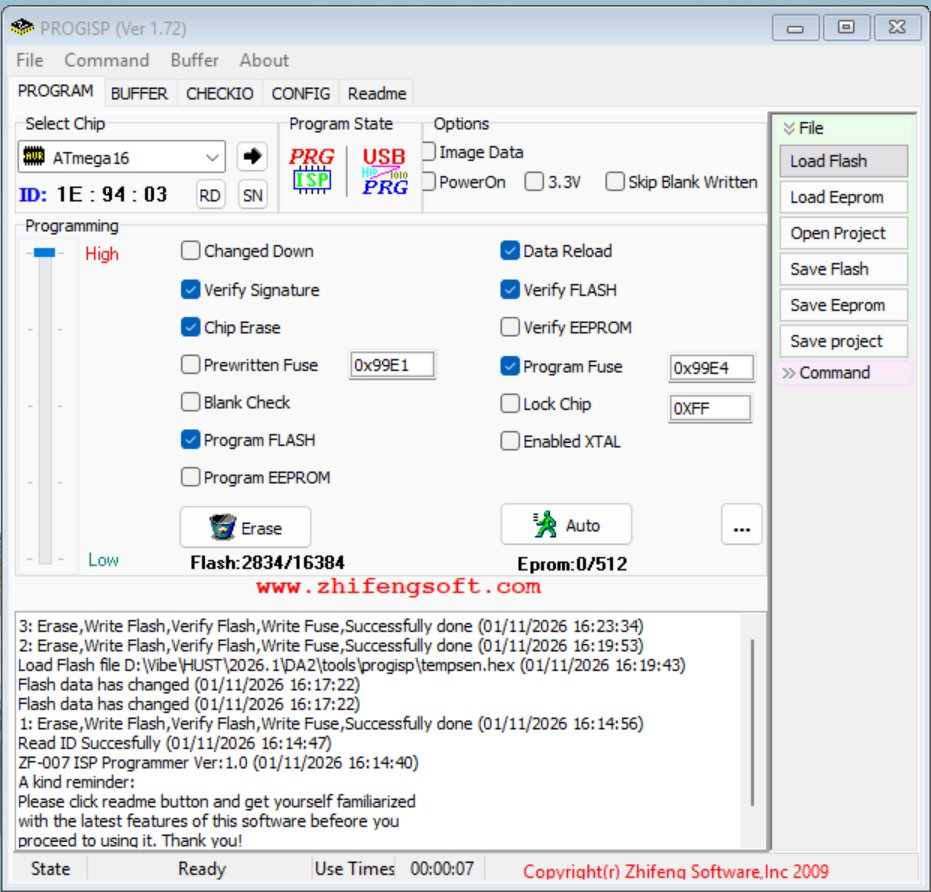
\includegraphics[width=0.72\textwidth,keepaspectratio]{progisp_setup.png}
\caption{Giao diện ProgISP khi nạp firmware và cấu hình fuse \texttt{0xD9E4}}
\label{fig:progisp-setup}
\end{figure}

\endgroup

\chapter{KẾT QUẢ THỰC NGHIỆM}

\section{Kết quả thực nghiệm trên phần cứng}
\label{sec:hw-results}

Hệ thống đo nhiệt độ và cảnh báo ngưỡng sử dụng vi điều khiển ATmega16 và cảm biến DHT11 đã được lắp ráp, nạp mã thực thi và kiểm thử thực tế trên Kit phát triển AVR tại phòng thí nghiệm Trường Điện -- Điện tử, Đại học Bách khoa Hà Nội. Các trạng thái chức năng ghi nhận trong quá trình thử nghiệm được tổng hợp dưới đây; phạm vi và giới hạn của phép kiểm chứng được trình bày ở mục \ref{sec:limitations}.

\subsection{Giai đoạn khởi động và màn hình chào mừng}
Khi vừa cấp nguồn nuôi 5V từ cổng nạp USB, vi điều khiển hoàn tất quá trình reset phần cứng, tắt cổng JTAG nội, thiết lập chiều cổng I/O và cấu hình màn hình LCD. Sau khi khởi tạo, màn hình LCD 1602 hiển thị thông điệp chào mừng khởi động:
\LCDbox{DA2: DO NHIET DO}{DHT11 SENSOR}
Màn hình duy trì thông điệp này trong khoảng 1,5 giây theo trễ phần mềm. Trong suốt giai đoạn khởi động, toàn bộ 5 đèn LED cảnh báo trên các chân PD0 -- PD4 đều tắt nhờ lệnh khởi tạo kéo mức 1 (\texttt{PORTD |= 0x1F}). Sau 1,5 giây, lệnh xóa màn hình (\texttt{0x01}) được phát ra để chuẩn bị cho chu trình hiển thị dữ liệu đo lường.

\subsection{\texorpdfstring{Trạng thái đo lường bình thường ($T < 30^\circ\text{C}$)}{Trạng thái đo lường bình thường (T < 30 °C)}}
Ở trạng thái không cảnh báo, giá trị được ghi nhận trên LCD là $26.5^\circ\text{C}$ (nhỏ hơn ngưỡng cài đặt $30^\circ\text{C}$):
\begin{itemize}[leftmargin=1.2cm]
    \item Cảm biến DHT11 thu thập dữ liệu và gửi gói tin 40-bit về MCU. Quá trình kiểm tra tính toàn vẹn dữ liệu bằng mã Checksum thành công, dữ liệu nhận được hợp lệ.
    \item \begin{samepage}Màn hình LCD 1602 hiển thị thông số:
    \LCDbox{Temp: 26.5 \textdegree C}{HIGH Th: 30\textdegree C}
    \end{samepage}
    \item Do giá trị nhiệt độ nhận được nhỏ hơn ngưỡng cài đặt, dòng 2 hiển thị ngưỡng \texttt{"HIGH Th: 30°C"} mà không xuất hiện bất kỳ dấu hiệu cảnh báo nào.
    \item Dàn 5 LED cảnh báo nối với các chân PD0 -- PD4 tiếp tục được giữ ở mức logic 1, nghĩa là tắt.
\end{itemize}

\subsection{\texorpdfstring{Trạng thái cảnh báo vượt ngưỡng quá nhiệt ($T \ge 30^\circ\text{C}$)}{Trạng thái cảnh báo vượt ngưỡng quá nhiệt (T ≥ 30 °C)}}
Để kiểm thử phản ứng của hệ thống khi có sự cố quá nhiệt, người thực hiện sử dụng nguồn nhiệt gián tiếp (hơi ấm nhẹ áp gần bề mặt cảm biến DHT11). Khi giá trị nhiệt độ nhận được đạt hoặc vượt $30.0^\circ\text{C}$:
\begin{itemize}[leftmargin=1.2cm]
    \item Vi điều khiển phát hiện điều kiện $temp\_int \ge 30^\circ\text{C}$ ở chu kỳ đọc hợp lệ tiếp theo (mỗi vòng lặp có trễ phần mềm 2 giây, cộng thời gian đọc và hiển thị).
    \item Màn hình LCD cập nhật trạng thái báo động tương ứng:
    \LCDbox{Temp: 31.5 \textdegree C}{HIGH Th: 30\textdegree C *!}
    Trên dòng 2 xuất hiện chuỗi ký hiệu báo động \texttt{"*!"} để báo cho người vận hành.
    \item Đồng thời, phép toán che mặt nạ \texttt{PORTD \&= 0xE0} kéo 5 chân PD0 -- PD4 xuống mức 0, làm 5 LED cảnh báo cùng sáng.
    \item Khi nguồn nhiệt được rút ra và giá trị nhiệt độ nhận được giảm trở lại dưới $30.0^\circ\text{C}$, màn hình tự động xóa ký hiệu \texttt{"*!"} và dàn đèn LED tự động tắt, trả hệ thống về trạng thái giám sát bình thường mà không cần thao tác reset thủ công.
\end{itemize}

\begin{figure}[H]
    \centering
    \begin{subfigure}[b]{0.46\textwidth}
        \centering
        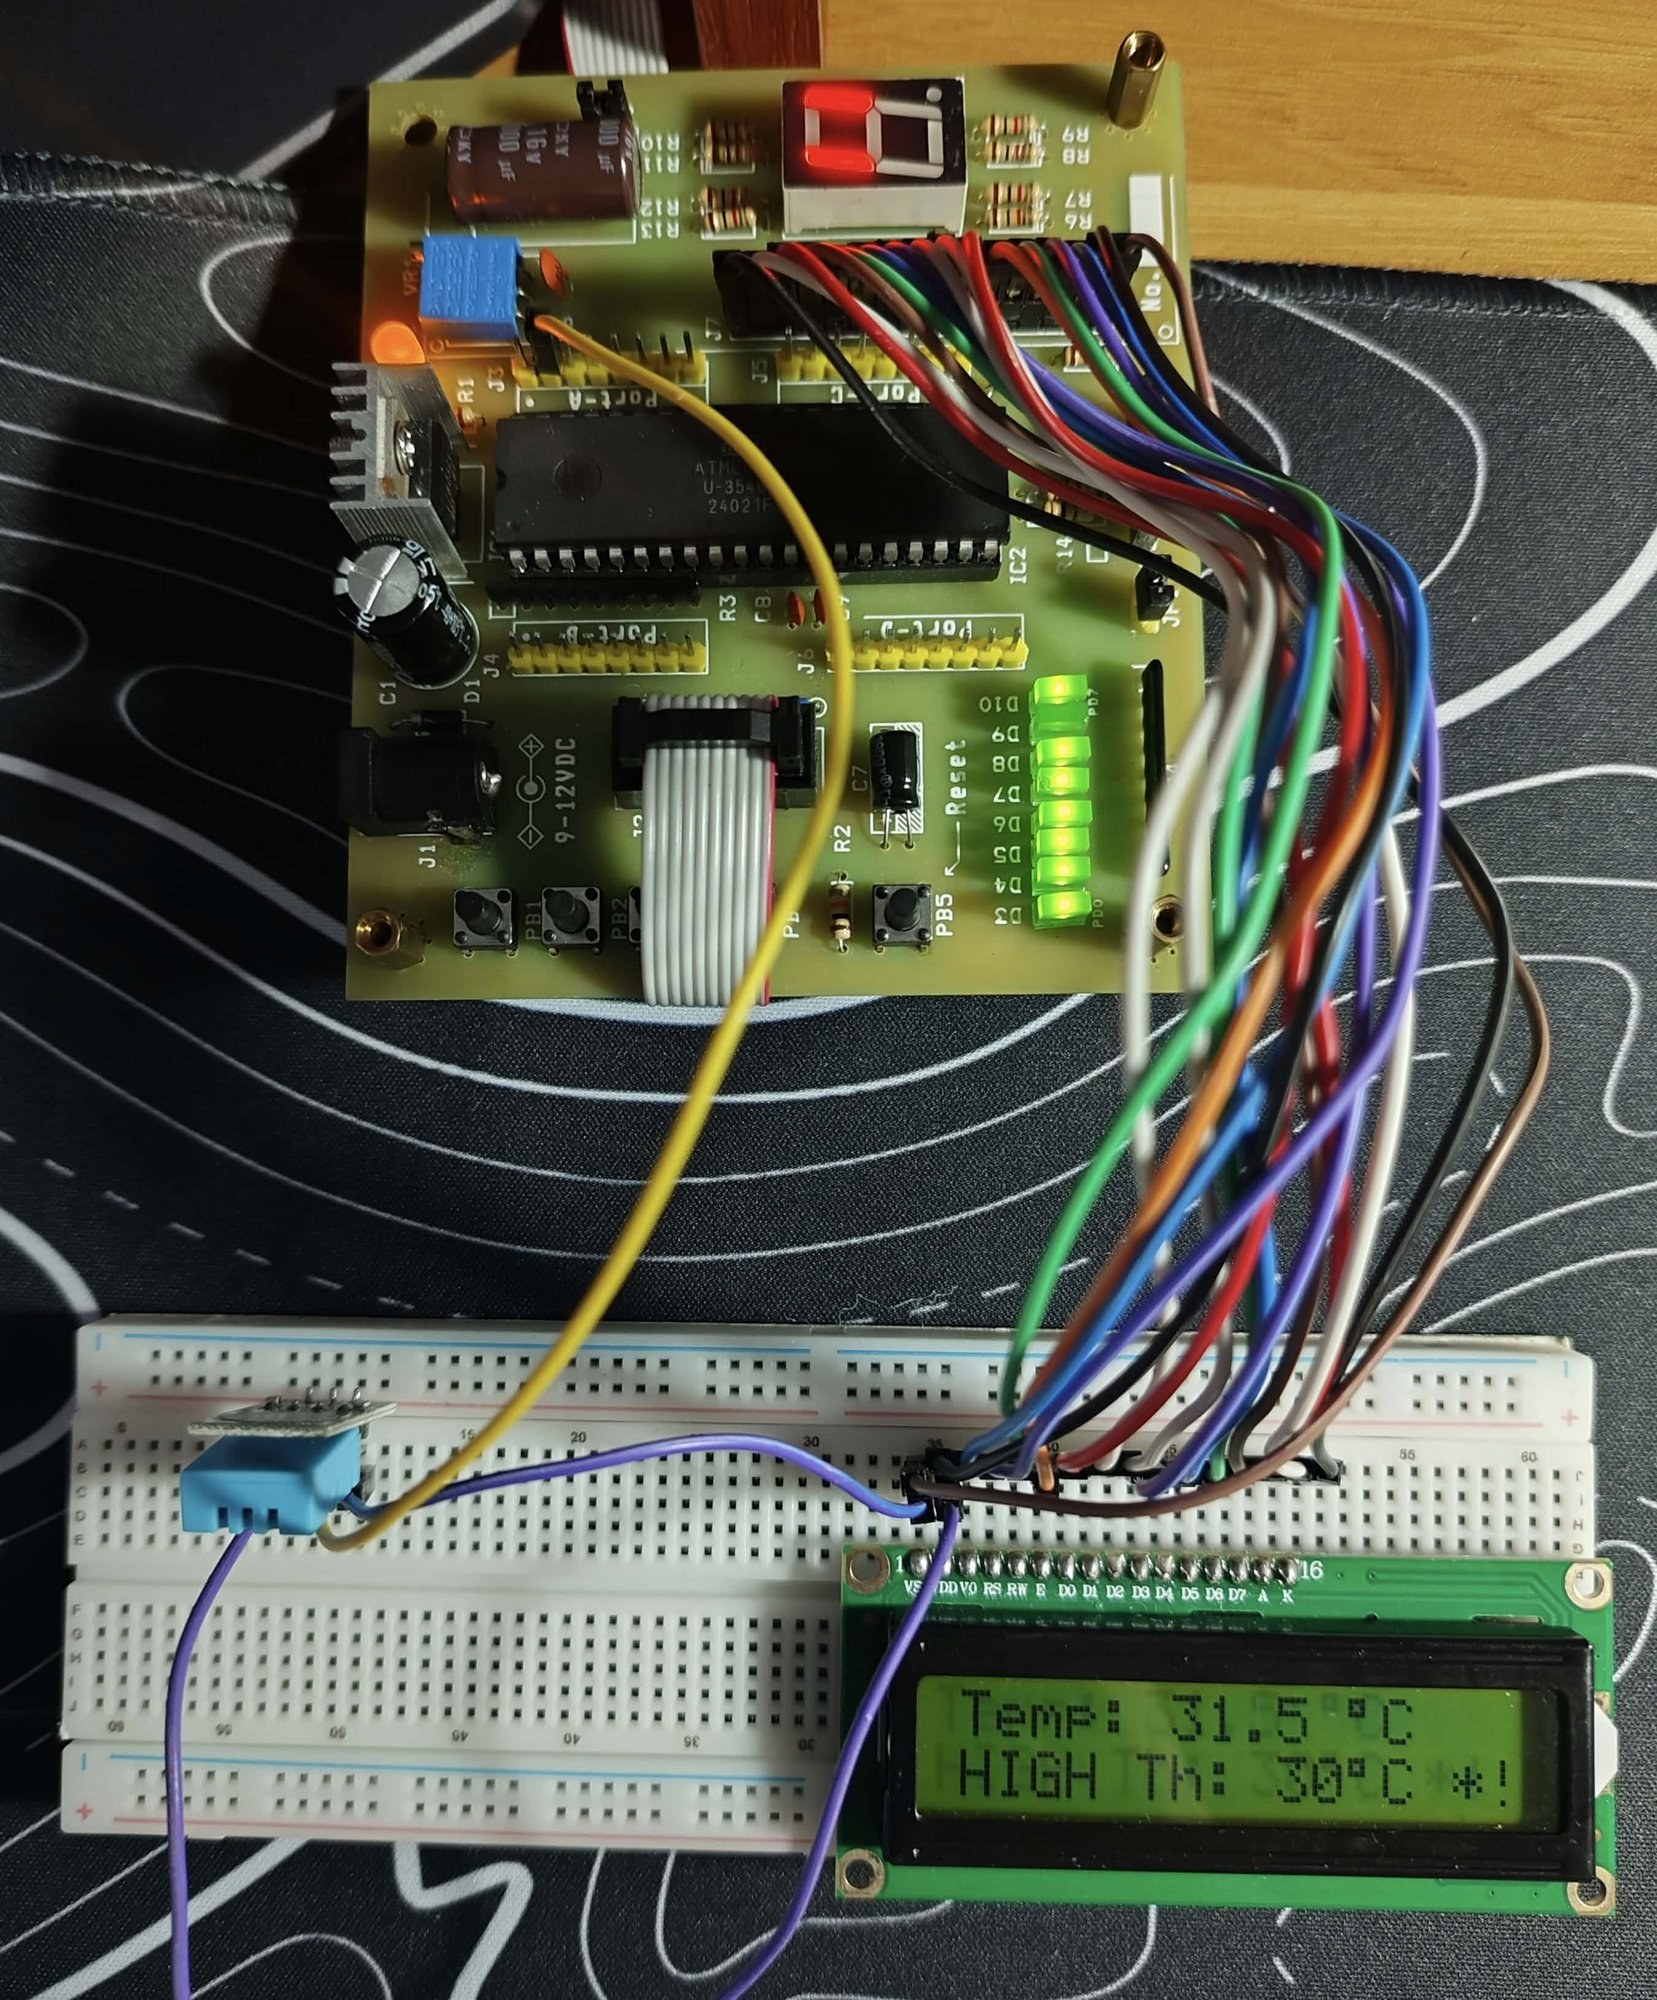
\includegraphics[height=7.5cm,keepaspectratio]{actual_system.jpg}
        \caption{Màn hình LCD khi cảnh báo quá nhiệt ($31.5^\circ\text{C}$)}
        \label{fig:actual-overheat}
    \end{subfigure}
    \hfill
    \begin{subfigure}[b]{0.46\textwidth}
        \centering
        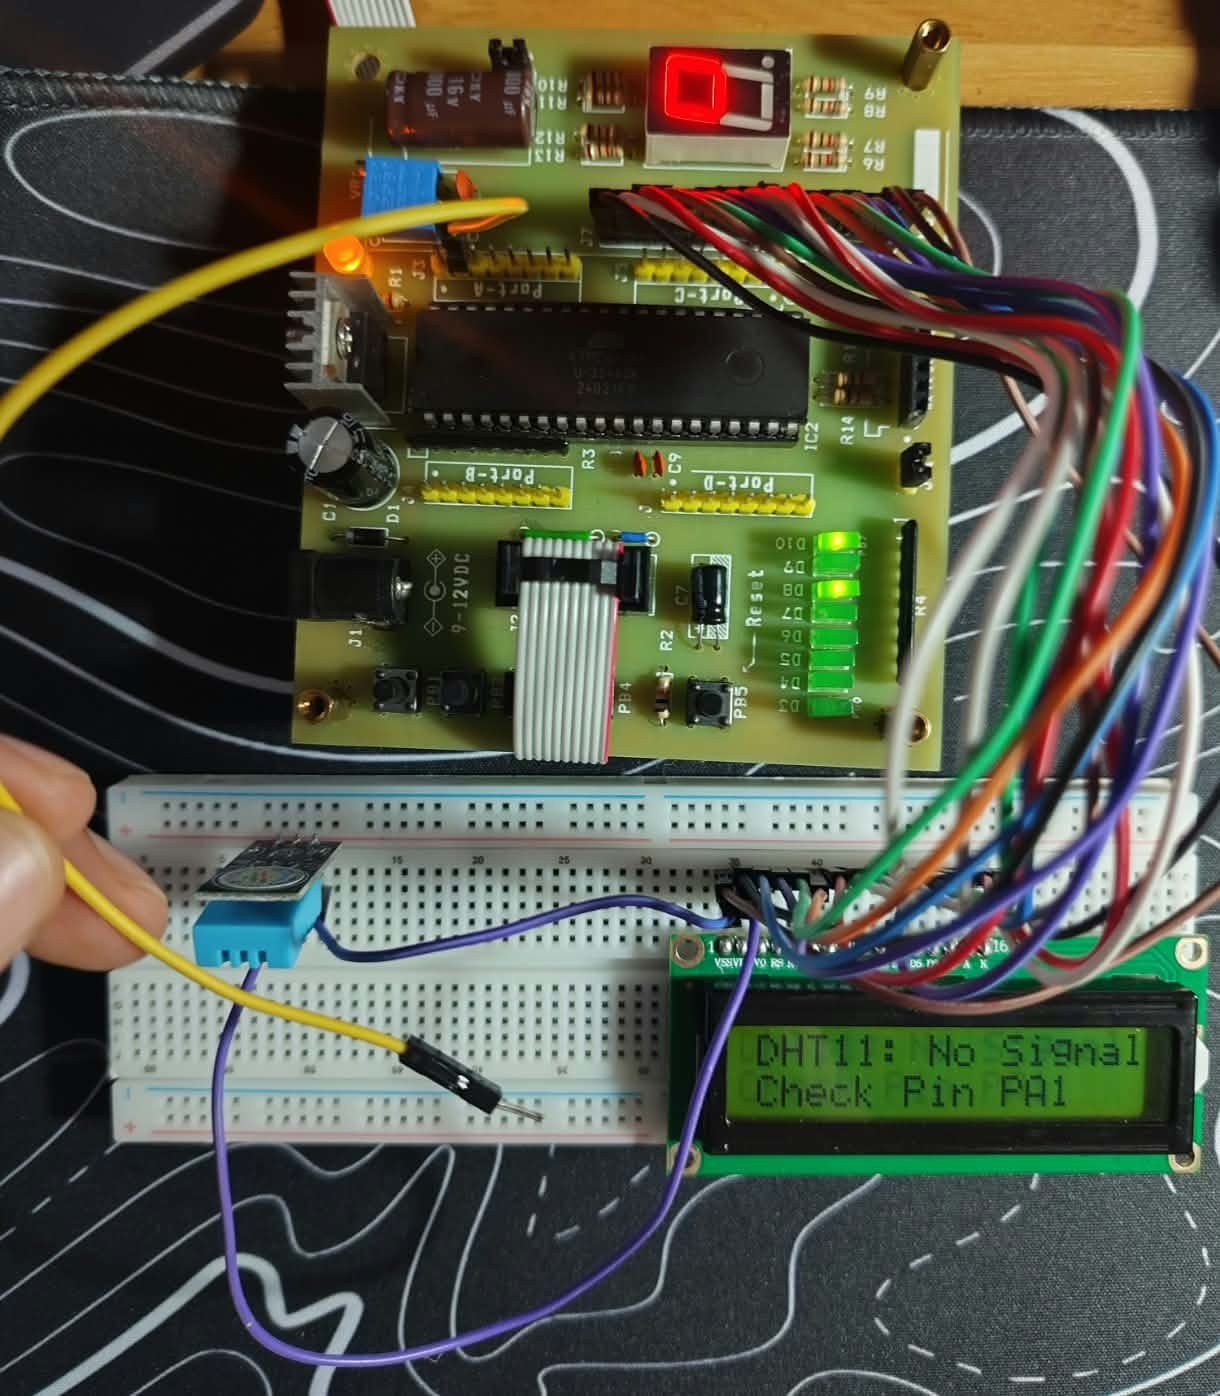
\includegraphics[height=7.5cm,keepaspectratio]{sensor_disconnect.jpg}
        \caption{Màn hình LCD khi không có tín hiệu từ cảm biến}
        \label{fig:actual-disconnect}
    \end{subfigure}
    \caption{Hình ảnh thực tế hệ thống vận hành trong các kịch bản thử nghiệm}
    \label{fig:actual-system}
    \vspace{0.1cm}
    {\small\textit{Ghi chú:} Dãy LED trên kit gồm 8 LED nối PD0--PD7 (từ D3 ở dưới lên D10 ở trên). Ba LED trên cùng (PD5--PD7) dùng chung đường RW, RS, EN của LCD nên sáng theo mức logic của các tín hiệu này, không thuộc khối cảnh báo. Ở (a), 5 LED cảnh báo PD0--PD4 sáng; ở (b), 5 LED này tắt.\par}
\end{figure}

\subsection{Kiểm tra phản hồi khi mất cảm biến và xử lý lỗi hệ thống}
Nhằm kiểm tra độ tin cậy và khả năng tự bảo vệ của hệ thống trước các tình huống bất thường, nhóm đã tiến hành xác minh theo hai cấp độ:
\begin{itemize}[leftmargin=1.2cm, topsep=0pt, itemsep=0.5pt, parsep=0pt]
    \item Thử nghiệm thực tế khi mất cảm biến (Kiểm chứng phần cứng): Để mô phỏng sự cố tuột dây tín hiệu, nhóm chủ động rút chân DATA (PA1). Vòng chờ đầu tiên của \texttt{DHT11\_Read} hết hạn và hàm trả về $-1$ sau khoảng 29\,ms (Bảng \ref{tab:timeout}); vi điều khiển không bị treo. Màn hình LCD cập nhật thông báo chẩn đoán lỗi sau khi hàm đọc cảm biến phát hiện timeout (Hình \ref{fig:actual-disconnect}):
    \LCDbox{DHT11: No Signal}{Check Pin PA1}
    \item Kiểm chứng giải thuật xử lý Checksum (Phân tích mã nguồn): Đối với trường hợp đường truyền bị can nhiễu, do chưa có thiết bị tạo xung nhiễu chuyên dụng, nhánh xử lý sai Checksum hiện chỉ được đối chiếu với luồng logic mã nguồn (nhánh \texttt{status == -6}). Thuật toán nhận diện sự sai lệch tổng kiểm tra và hiển thị thông báo chuẩn 16 ký tự:
    \LCDbox{DHT11: Sum Error}{Checksum Invalid}
    \item Trạng thái xử lý lỗi xác định: Trong cả hai tình huống, dàn 5 LED được đưa về trạng thái tắt (\texttt{PORTD |= 0x1F}) như phân tích ở mục \ref{sec:main-algo}.
\end{itemize}

\begin{table}[H]
\centering
\small
\setlength{\tabcolsep}{3pt}
\caption{Bảng tổng hợp các kịch bản kiểm tra và kết quả đánh giá hệ thống}
\label{tab:system-results}
\renewcommand{\arraystretch}{1.15}
\begin{tabularx}{\textwidth}{>{\bfseries\raggedright\arraybackslash}p{2.6cm} >{\raggedright\arraybackslash}p{2.6cm} >{\centering\arraybackslash}p{1.5cm} >{\raggedright\arraybackslash}X >{\centering\arraybackslash}p{1.8cm}}
\toprule
\textbf{Kịch bản kiểm tra} & \textbf{Phương pháp xác minh} & \textbf{Giá trị LCD} & \textbf{Nội dung hiển thị trên LCD 1602} & \textbf{Trạng thái dàn LED} \\
\midrule
Khởi động hệ thống & Thực nghiệm trên kit & -- & Dòng 1: \mbox{\texttt{DA2: DO NHIET DO}}\newline Dòng 2: \mbox{\texttt{DHT11 SENSOR}} & Tắt toàn bộ \\
\midrule
Nhiệt độ bình thường & Thực nghiệm trên kit & $26.5^\circ\text{C}$ & Dòng 1: \mbox{\texttt{Temp: 26.5 \textdegree C}}\newline Dòng 2: \mbox{\texttt{HIGH Th: 30\textdegree C}} & Tắt toàn bộ \\
\midrule
Nhiệt độ vượt ngưỡng & Thực nghiệm trên kit & $31.5^\circ\text{C}$ & Dòng 1: \mbox{\texttt{Temp: 31.5 \textdegree C}}\newline Dòng 2: \mbox{\texttt{HIGH Th: 30\textdegree C *!}} & Bật sáng cả 5 LED \\
\midrule
Mất tín hiệu cảm biến & Thực nghiệm trên Kit (Rút chân PA1) & -- & Dòng 1: \mbox{\texttt{DHT11: No Signal}}\newline Dòng 2: \mbox{\texttt{Check Pin PA1}} & Tắt toàn bộ (Xác định) \\
\midrule
Sai mã Checksum & Phân tích giải thuật mã nguồn & -- & Dòng 1: \mbox{\texttt{DHT11: Sum Error}}\newline Dòng 2: \mbox{\texttt{Checksum Invalid}} & Tắt toàn bộ (Xác định) \\
\bottomrule
\end{tabularx}
\end{table}

\section{Đánh giá kết quả và phạm vi kiểm chứng}

\subsection{Kết quả chức năng đã ghi nhận}
Các mô tả và ảnh ở mục \ref{sec:hw-results} cho thấy chương trình có thể hiển thị giá trị nhiệt độ, báo vượt ngưỡng bằng LCD và LED, đồng thời hiển thị thông báo khi mất tín hiệu cảm biến. Bảng \ref{tab:system-results} phân biệt kịch bản thử trên phần cứng với nhánh checksum mới được xem xét qua mã nguồn. Phân tích mã nguồn cho thấy điều kiện \texttt{temp\_int >= 30} bao gồm cả trường hợp đúng ngưỡng; báo cáo hiện chưa có kết quả thử riêng tại $30^\circ\text{C}$.

Hình \ref{fig:actual-system}a ghi nhận LCD hiển thị $31.5^\circ\text{C}$ cùng ký hiệu \texttt{*!} và 5 LED cảnh báo sáng. Vì chương trình in trực tiếp $T_{int}$ và $T_{dec}$ nhận từ cảm biến, phần thập phân \texttt{.5} trên LCD chính là giá trị Byte 3 của gói tin: module đang dùng trả về byte thập phân khác 0, khác với bản tài liệu tham chiếu ghi độ phân giải $1^\circ\text{C}$ \cite{dht11-datasheet}. Các giá trị này phản ánh dữ liệu cảm biến gửi về; độ chính xác so với nhiệt độ môi trường cần được đối chiếu thêm với nhiệt kế tham chiếu.

\begin{samepage}
Checksum chỉ xác nhận gói tin được truyền đúng, không xác nhận độ chính xác vật lý của phép đo. Khi có lỗi, chương trình tắt 5 LED và hiển thị chẩn đoán; vì vậy LED tắt không đủ để kết luận môi trường đang dưới ngưỡng.
\par\end{samepage}

\subsection{Giới hạn của kết quả thực nghiệm}
\label{sec:limitations}
Báo cáo hiện chưa có các dữ liệu sau để đánh giá định lượng:
\begin{itemize}[leftmargin=1.2cm]
    \item Các cặp số đo đồng thời giữa hệ thống và nhiệt kế tham chiếu tại nhiều mức nhiệt, nên chưa xác định được sai lệch trung bình hoặc sai lệch lớn nhất.
    \item Nhật ký chạy liên tục gồm tổng số lần đọc, số lần hợp lệ, số lỗi timeout và checksum, nên chưa tính được tỷ lệ đọc thành công hoặc độ ổn định dài hạn.
    \item Thời gian từ khi số đo chạm ngưỡng đến khi LED đổi trạng thái; trễ 2 giây trong mã nguồn không thể thay thế phép đo độ trễ toàn hệ thống.
    \item Thử lặp lại tại dưới ngưỡng, đúng ngưỡng và trên ngưỡng, cũng như thao tác rút rồi nối lại cảm biến khi hệ thống đang cảnh báo.
\end{itemize}
Kết quả hiện có hỗ trợ đánh giá chức năng cơ bản, chưa xác nhận độ chính xác đo hoặc độ tin cậy dài hạn.

\chapter{KẾT LUẬN VÀ HƯỚNG PHÁT TRIỂN}

\section{Kết luận}

Đề tài đã triển khai mô hình đo nhiệt độ và cảnh báo ngưỡng trên nền tảng ATmega16, DHT11 và LCD 1602. Các kết quả chính gồm:
\begin{itemize}[leftmargin=1.2cm]
    \item Vẽ lại sơ đồ nguyên lý từ tài liệu giảng viên cung cấp và thiết kế PCB trên Altium Designer; xác định kết nối cảm biến ngoài kit và các nhóm chân dùng cho LCD, LED.
    \item Triển khai chương trình C đọc gói dữ liệu 40-bit từ DHT11, kiểm tra checksum, giới hạn mỗi vòng chờ bằng timeout 7,5--8,75\,ms và phân loại thông báo lỗi. Chương trình chiếm 2830 B (17,3\,\%) bộ nhớ Flash.
    \item Cấu hình thư viện LCD giao tiếp 4-bit và mặt nạ bit để cập nhật LCD, LED trên các nhóm chân dùng chung cổng D.
    \item Thống nhất cấu hình RC nội 8 MHz, fuse \texttt{0xD9E4}, giá trị \texttt{F\_CPU} và thao tác vô hiệu hóa JTAG nhằm sử dụng PC4, PC5 cho LCD.
    \item Ghi nhận các trạng thái hiển thị nhiệt độ, cảnh báo ngưỡng và báo mất tín hiệu cảm biến như Chương 3. Nhánh lỗi checksum hiện được đối chiếu bằng phân tích mã nguồn.
\end{itemize}
Mô hình đã thực hiện đúng các chức năng đề ra trong phạm vi thử nghiệm đã trình bày; các hạn chế còn lại được tổng hợp ở mục \ref{sec:conclusion-limits}.

\section{Hạn chế của đề tài}
\label{sec:conclusion-limits}

Các hạn chế hiện tại của mô hình gồm:
\begin{itemize}[leftmargin=1.2cm]
    \item Cảm biến DHT11 có dải đo nhiệt độ hẹp ($0^\circ\text{C} - 50^\circ\text{C}$) và sai số tương đối lớn ($\pm 2.0^\circ\text{C}$), chu kỳ lấy mẫu tương đối chậm (chương trình chèn trễ 2 giây sau mỗi vòng lặp) nên chưa phù hợp cho các môi trường đòi hỏi đáp ứng thời gian thực cực nhanh.
    \item Chưa có phép đo đối chiếu với nhiệt kế tham chiếu, nhật ký chạy dài hạn và phép đo độ trễ cảnh báo, nên độ chính xác và độ ổn định của hệ thống mới được đánh giá ở mức chức năng (mục \ref{sec:limitations}).
    \item Chưa có hysteresis, nên cảnh báo có thể đổi trạng thái nhiều lần khi số đo dao động quanh ngưỡng.
    \item Ngưỡng cảnh báo nhiệt độ ($30^\circ\text{C}$) hiện đang được cố định cứng trong mã nguồn, người sử dụng chưa thể linh hoạt thay đổi ngưỡng trực tiếp từ bên ngoài bằng phím bấm mà phải biên dịch lại chương trình.
    \item Cơ chế xử lý khi mất cảm biến hiện đưa toàn bộ LED về trạng thái tắt để tránh báo động giả từ dữ liệu cũ lỗi thời, nhưng có nhược điểm là không tiếp tục cảnh báo bằng đèn nếu môi trường thực tế vẫn đang quá nhiệt.
    \item Hệ thống chưa có bộ nhớ lưu trữ lịch sử biến thiên nhiệt độ theo thời gian và chưa có khả năng truyền thông dữ liệu từ xa lên mạng máy tính.
\end{itemize}

\section{Hướng phát triển mở rộng}
\label{sec:future}

Từ mô hình phần cứng và phần mềm hiện có, hệ thống có thể tiếp tục được nghiên cứu và nâng cấp theo các hướng ứng dụng thực tế:
\begin{enumerate}[leftmargin=1.2cm]
    \item Hoàn thiện kiểm chứng: thu log dữ liệu thô, đối chiếu nhiệt kế tham chiếu, thống kê lỗi khi chạy liên tục và đo độ trễ. Bổ sung hysteresis với ngưỡng bật/tắt riêng theo yêu cầu ứng dụng và độ biến động của số đo.
    \item Nâng cấp cảm biến: Thay thế cảm biến DHT11 bằng các dòng cảm biến kỹ thuật số có độ chính xác cao hơn phù hợp với yêu cầu ứng dụng; các phương án có thể khảo sát gồm DHT22, cảm biến I2C như Sensirion SHT30/SHT35 hoặc Bosch BME280 (đo đồng thời nhiệt độ, độ ẩm và áp suất khí quyển).
    \item Bổ sung giao diện người dùng tương tác linh hoạt: Tích hợp bàn phím ma trận $4 \times 4$ hoặc cụm nút bấm tăng/giảm/cài đặt kết hợp còi báo, cho phép người dùng tự do cài đặt ngưỡng nhiệt độ cảnh báo và lưu trữ giá trị cấu hình này vào bộ nhớ không biến động EEPROM của ATmega16.
    \item Bổ sung chế độ cảnh báo lỗi cảm biến chuyên biệt: Lập trình cơ chế nhấp nháy toàn bộ dàn LED (tần số 2 Hz) hoặc còi buzzer ngắt quãng khi mất kết nối cảm biến để người vận hành phân biệt rõ ràng giữa trạng thái "Bình thường" (LED tắt), "Cảnh báo quá nhiệt" (LED sáng liên tục) và "Lỗi cảm biến" (LED nhấp nháy).
    \item Tích hợp kết nối không dây và phát triển ứng dụng IoT: Kết nối cổng giao tiếp nối tiếp USART của ATmega16 với các mô-đun truyền thông không dây như Wi-Fi ESP8266/ESP32, Bluetooth HC-05 hoặc chuẩn truyền xa LoRa để gửi dữ liệu nhiệt độ lên máy chủ đám mây qua giao thức MQTT/HTTP. Qua đó, người quản lý có thể giám sát biểu đồ nhiệt độ môi trường và nhận thông báo cảnh báo khẩn cấp trực tiếp trên ứng dụng điện thoại thông minh (Blynk, ThingsBoard) qua kết nối mạng. Khi dùng USART phần cứng, cần bố trí lại LED trên PD0/RXD và PD1/TXD để tránh xung đột chức năng, đồng thời kiểm tra mức điện áp giao tiếp của module.
\end{enumerate}

\begin{thebibliography}{99}
\addcontentsline{toc}{chapter}{TÀI LIỆU THAM KHẢO}

\bibitem{atmega16-datasheet}
Atmel Corporation, ``ATmega16/ATmega16L 8-bit AVR Microcontroller with 16K Bytes In-System Programmable Flash Datasheet'', Document Rev. 2466T--AVR--07/10, San Jose, CA, USA, 2010.

\bibitem{dht11-datasheet}
Aosong Electronics Co., Ltd, ``DHT11 Humidity \& Temperature Sensor Product Manual'', Guangzhou Aosong Electronics Co., Ltd, Guangzhou, China, 2015.

\bibitem{hd44780-datasheet}
Hitachi Semiconductor and Integrated Circuits, ``HD44780U (Dot Matrix Liquid Crystal Display Controller/Driver) Technical Data'', Rev. 0.0, Tokyo, Japan, 1998.

\bibitem{hust-kit-manual}
Trường Điện -- Điện tử (Viện Điện tử -- Viễn thông), Đại học Bách khoa Hà Nội, ``Tài liệu hướng dẫn thực hành và sơ đồ nguyên lý Kit vi điều khiển AVR ATmega16'', Hà Nội, 2022.

\bibitem{ngo-dien-tap}
Ngô Diên Tập, ``Kỹ thuật vi điều khiển và ứng dụng -- Lập trình họ vi điều khiển AVR'', Nhà xuất bản Khoa học và Kỹ thuật, Hà Nội, 2012.

\bibitem{avrgcc-manual}
Free Software Foundation, ``AVR-GCC and AVR Libc User Manual -- A C runtime library for Atmel AVR microcontrollers'', \url{https://www.nongnu.org/avr-libc/}, truy cập tháng 10/2026.

\bibitem{seee-report-guide}
Trường Điện -- Điện tử, Đại học Bách khoa Hà Nội, ``Quy định về thể thức văn bản và cấu trúc báo cáo Đồ án môn học -- Đồ án tốt nghiệp bậc đại học'', Hà Nội, 2023.

\end{thebibliography}

\chapter*{PHỤ LỤC: TOÀN BỘ MÃ NGUỒN CHƯƠNG TRÌNH}
\addcontentsline{toc}{chapter}{PHỤ LỤC: TOÀN BỘ MÃ NGUỒN CHƯƠNG TRÌNH}

\section*{Phụ lục A: File mã nguồn chính \texttt{tempsen.c}}
\VerbatimInput[fontsize=\footnotesize,baselinestretch=1.05,breaklines=true,breakanywhere=true,tabsize=4]{../../../src/tempsen.c}

\section*{Phụ lục B: Thư viện điều khiển LCD \texttt{hunget\_lcd.h}}
\VerbatimInput[fontsize=\footnotesize,baselinestretch=1.05,breaklines=true,breakanywhere=true,tabsize=4]{../../../src/hunget_lcd.h}


\end{document}
